\documentclass[uplatex,dvipdfmx]{jsarticle}
\usepackage{listings,jvlisting}
\usepackage{color}
\usepackage{xr}

\lstset{
  backgroundcolor=\color[rgb]{0.9,0.9,0.9},
  frame=single,
  basicstyle=\ttfamily
}
\makeatletter
\newcommand*{\addFileDependency}[1]{% argument=file name and extension
  \typeout{(#1)}
  \@addtofilelist{#1}
  \IfFileExists{#1}{}{\typeout{No file #1.}}
}
\makeatother

\newcommand*{\myexternaldocument}[1]{%
    \externaldocument{#1}%
    \addFileDependency{#1.tex}%
    \addFileDependency{#1.aux}%
}
\myexternaldocument{../categoryTheoryIntro/CategoryTheoryIntro}

\newcommand{\pr}[1]{\colorbox[rgb]{0.9,0.9,0.9}{\lstinline{#1}}}
\newcommand{\functype}[2]{\pr{#1 -> #2}}
\newcommand{\refcti}[1]{[CTI]\ref{#1}}
\newcommand{\fpmor}[3]{\pr{#1 :: #2 -> #3}}
\input{../categoryTheoryIntro/preemble.tex}
\begin{document}
  \title{Profunctor Opticsの理論と実装}
  \author{https://otamusan.github.io/FPandCategory/categoricalfp.pdf}
  \maketitle
	\tableofcontents
  \pagebreak
  \section{Haskellの基礎}
  \subsection{関数型}
  Haskellにも一般のプログラミングと同じようにデータ型が存在し、整数値を持つ\pr{Int}型や\pr{True}と\pr{False}を持つ\pr{Bool}型などがある。
  また整数値を受け取って二倍にして返す、つまり$double(x)=2x$なる
  関数\pr{double}は\pr{Int}から\pr{Int}への関数であり、haskellではこのように記述する。
  \begin{lstlisting}
    double :: Int -> Int
    double x = 2*x
    -- >>> double 4
    -- 8
  \end{lstlisting}
  ある型\pr{a}からある型\pr{b}への関数は、関数の型\functype{a}{b}に含まれる。すなわち、関数そのものも値とみなすということである。それによって、関数型から関数型への関数なども定義できるようになる。その一例を示そう。

  関数\fpmor{f}{Int}{Int}を、自身を合成した関数\fpmor{f.f}{Int}{Int}へと写す関数
  
  \fpmor{mul}{(Int -> Int)}{(Int -> Int)}は次のように記述する。
  \begin{lstlisting}
    mul :: (Int -> Int) -> (Int -> Int)
    mul f = f.f
    -- >>> (mul double) (5)
    -- 20
  \end{lstlisting}
  後に説明するが、\pr{.}という記号は前後の関数を合成する操作であり、\pr{f.f}は$f\circ f$を意味する。すなわちこの計算は
  \[(mul(double))(5)=(double \circ double)(5)=double(double(5))=20\]のように行われる。このような関数を引数、戻り値にするような関数を高階関数と呼ぶ。
  
  二つの整数を足し合わせる操作は$add(x,y)=x+y$のように定義できる。この関数は引数を二つ持つ多変数関数であり、これはHaskellでは
  \begin{lstlisting}
    add :: Int -> Int -> Int
    add x y = x + y
    -- >>> add 5 6
    -- 11
  \end{lstlisting}
  のように型を与えて定義することができる。関数の型\pr{Int -> Int -> Int}は左から二つは引数の型で、一番右が返り値の型となっている。
  なぜこのような表記をするかというと、\pr{Int -> Int -> Int}は\pr{Int -> (Int -> Int)}の省略であり、$add(x,y)$を$(add(x))(y)$とみなしているためである。ゆえに\fpmor{add(x)}{Int}{Int}は引数に\pr{x}を足し合わせる関数となっている。またこのように想定された数より少ない引数を適用することを部分適用と呼ぶ。
  \subsection{多相型と多相関数}
  関数型\functype{a}{b}は単一の型ではなく、任意の型\pr{a},\pr{b}に対して個別に定義できるのであった。このように既存の型から生成できる型を多相型という。また、多相型から多相型への型を考えることもできる。例えば高階関数と多変数関数を用いれば、関数を合成する操作に次のような型を与えることができる。
  \begin{lstlisting}
    apply :: (Int -> Int) -> Int -> Int
    apply f x = f(x)
    -- >>> apply double 10
    -- 20
  \end{lstlisting}
  しかし、引数の関数は\pr{Int}か\pr{Int}への関数に制限されているが、実際は関数がどのような型であっても、適用の操作は行えるはずである。
  そこで、\pr{apply}関数の引数の型を\pr{a}、返り値の型を\pr{b}に置き換える。
    \begin{lstlisting}
    apply :: (a -> b) -> a -> b
    apply f x = f(x)
    -- >>> apply double 10
    -- 20
    -- >>> apply not False
    -- True
  \end{lstlisting}
  例のために真理値を反転する関数\fpmor{not}{Bool}{Bool}を使用している。
  
  このように関数の引数の型を任意の型\pr{a},\pr{b}に置き換えることで、様々な型の値に対応した関数を定義することができ、このような関数を多相関数と呼ぶ。

  このような多相関数は基本的に既存の多相関数の組み合わせによって定義される。この例であれば、\pr{apply}の定義に用いた\pr{f(x)}はすでにhaskell側によって多相関数\pr{(\$) :: (a -> b) -> a -> b}としてすでに定義されているため、定義することができた。

  値の適用が関数として与えられているように、関数の合成も関数で行うことができる。つまり関数\pr{double}の定義に用いた\pr{.}が関数であり、
  \begin{center}
    \pr{(.)\ ::\ (b -> c) -> (a -> b) -> a -> c}
  \end{center}
  という型が与えられているということである。

  このように関数型プログラミングでの処理の記述は変数の仲介を除けば、関数に関数を合成する操作や、関数に値を適用する操作によって行われる。
  \subsection{基本的なデータ型}
  任意の型\pr{a},\pr{b}に対して多相型である直積型\pr{(a,b)}は以下の関数で構成される。
  \begin{lstlisting}
    (,) :: a -> b -> (a, b)
    fst :: (a, b) -> a
    snd :: (a, b) -> b

    -- >>> (,) 4 5
    -- (4,5)
    -- >>> fst (4,5)
    -- 4
    -- >>> snd (4,5)
    -- 5
  \end{lstlisting}
  実行例を見て分かるように、\pr{(a,b)}の値はある型\pr{a}と\pr{b}の値をそれぞれ持つ。
  また、型\pr{a},\pr{b}の値\pr{x},\pr{y}に対して、\[\pr{fst (x, y)}=\pr{x},\ \pr{snd (x, y)}=\pr{y}\]が成り立つ。

  直積型は二つの型の値を持つが、ゼロ個の型の値を持つ型も存在する。この型をUnit型\pr{()}といい、ただ一つの値\pr{()}を持つ。

  任意の型\pr{a},\pr{b}に対して多相型である直和型\pr{Either a b}は以下の関数で構成される。
  \begin{lstlisting}
    Right :: b -> Either a b
    Left :: a -> Either a b
    either :: (a -> c) -> (b -> c) -> Either a b -> c

    isZero :: Int -> Bool
    isZero x = x==0

    -- >>> either isZero not (Left 0)
    -- True
    -- >>> either isZero not (Right True)
    -- False
  \end{lstlisting}
  \pr{isZero}関数の\pr{x==0}は両辺が等しいか真理値を返す関数\pr{(==)\ ::\ Int\ ->\ Int\ ->\ Bool}であり、定義から分かるように\pr{Either a b}は\pr{a}か\pr{b}の値のどちらか一方を持つ。

  \pr{either}関数についてこの例では、\functype{Int}{Bool}と\functype{Bool}{Bool}を受け取っているため、次の引数の型は\pr{Either\ Int\ Bool}を受け取る。もし\pr{Either\ Int\ Bool}の値が\pr{Int}であれば、\functype{Int}{Bool}型の\pr{isZero}関数に適用し、\pr{Bool}であれば\functype{Bool}{Bool}型の\pr{not}関数に適用する、という関数である。

  また任意の型\pr{x}とその値\pr{y}、
  \begin{lstlisting}
    f :: a -> x
    g :: b -> x
  \end{lstlisting}に対して、
  \begin{align*}
    \pr{either f g (Left x)}&=\pr{f x}\\
    \pr{either f g (Right x)}&=\pr{g x}
  \end{align*}
  が成り立つ。

  一般に直和を用いて新しい型を定義する場合、\pr{Either}型を用いて定義するのではなく、haskellにおける多相型を定義する構文によって行われることが多い。また\pr{either}関数もパターンマッチと呼ばれる構文によって行われる。

  \begin{lstlisting}
    data EitherIB = Value Int | Judge Bool
    calc :: EitherIB -> Bool
    calc (Value a) = isZero a
    calc (Judge a) = not a
    -- >>> :t Value
    -- Value :: Int -> EitherIB
    -- >>> :t Judge
    -- Judge :: Bool -> EitherIB
  \end{lstlisting}
  この例では、\pr{EitherIB}が\pr{Either Int Bool}に該当し、\pr{Value}が\pr{Left}、\pr{Judge}が\pr{Right}に対応する。
  \subsection{Haskellにおける型の応用}
  最後にこれらを応用したMaybe型を見る。
  \begin{lstlisting}
    data Maybe a  =  Nothing | Just a
  \end{lstlisting}
  \pr{Maybe a}は\pr{Either}型を用いると、\pr{Either () a}と書ける。ここでの\pr{Nothing}は\pr{Unit}型の値を与える関数とみなせるが、値はただ一つであるため単に定数と見て良い。すなわち\pr{Maybe a}はただ一つの値\pr{Nothing}と型\pr{a}の値のどちらかの値を持つ型である。

  この\pr{Maybe}の想定している用途として、以下の例を扱う。
  \begin{lstlisting}
    div10 :: Float -> Float
    div10 = (10 /)
    -- >>> div10 4
    -- 2.5
    -- >>> div10 0
    -- Infinity
  \end{lstlisting}
  \pr{div10}は10を与えられた数で割る関数であるが、結果のように零除算についてはInfinityという値が与えられる。これを素直に計算の失敗と見なし、型によって計算結果が正しく出力されないことを示したい。そこで、
  \begin{lstlisting}
    div10' :: Float -> Maybe Float
    div10' x = if x == 0 then Nothing else Just $ div10 x

    -- >>> div10' 4
    -- Just 2.5
    -- >>> div10' 0
    -- Nothing
  \end{lstlisting}


  という関数を定義する。これは零除算が発生する場合\pr{Nothing}を返し、そうでない場合は\pr{Just}によって計算結果を\pr{Maybe}に包んで返している。

  これによって、\pr{Maybe Float}の値を用いて計算を行うときは、必ず\pr{Nothing}と\pr{Just}の場合分けが必要になり、他の言語でいうNullチェックが必要なことを型レベルで示していることになる。
  \section{圏論}
  関数型言語では関数という言葉が使われるように、型を属する値の集合、関数を値の集合から値の集合への写像とみなすことができる。集合を写像の視点から観察する場合、圏論によって一般化することが有効である場合が多い。そのため以降は型と関数の議論を圏論によってモデル化することを考える。
  \subsection{型と関数の圏}
  型を対象、関数を射とする圏$\cat{H}$を定義する。
  圏の定義の詳細は\refcti{def-category}を参照
  Haskellには二つの関数が等しいことを判定する一般的な操作は無い。そのため関数の等号を改めて定義する。
  \begin{define}[関数の外延性]\label{def-function-extensionality}
    関数\fpmor{f}{a}{b}、\fpmor{g}{a}{b}と型\pr{a}の任意の値\pr{x}において\[\pr{f x}=\pr{g x} \iff \pr{f} = \pr{g}\]
  \end{define}
  \begin{define}[型と関数の圏]\label{def-hask-category}
		\begin{quote}~
			\begin{mydescription}
        \item[対象] すべての型の集合を対象集合$\obj{H}$とする。また各型を対象とみなす場合$A,B,C\cdots$と表記し、型とみなす場合は\pr{a},\pr{b},\pr{c}$\cdots$とする。また各型の値を圏論の文脈では$a,b,c\cdots$と表記することにする。
        \item[射] 対象$A$から対象$B$への射集合$\arset{H}{A}{B}$を集合と見なした関数型\functype{a}{b}とする。また各射は$f,g,h\cdots$と表記する。
        \item[射の合成] 射の合成を行う写像$\mor{\circ}{\arset{H}{B}{C}\times\arset{H}{A}{B}}{\arset{H}{A}{C}}$を任意の射$\mor{f}{A}{B},\ \mor{g}{B}{C}$に対して\pr{f.g}によって定義する。
        \item[恒等射の存在] 任意の型\pr{a}に対して恒等関数\fpmor{id}{a}{a}は、\pr{id x = x}と定義できる。この恒等関数を恒等射とし、$\mor{id_A}{A}{A}$と表記する。
        \item[結合律] 関数の外延性より、集合の圏における結合律と同様の手法で証明できる。\refcti{def-category-of-sets}を参照
        \item[単位元律]結合律と同様に\refcti{def-category-of-sets}を参照
		  \end{mydescription}
		\end{quote}
	\end{define}
  次に型の直積と直和の普遍性との関係を見る。
  \begin{prop}[$\cat{H}$の積]\label{prop-h-has-product}
    圏$\cat{H}$は積を持つ
  \end{prop}
  \begin{proof}
    $(\pr{(a,\ b)},\pr{fst},\pr{snd})$は型\pr{a},\pr{b}における積であることを示せば良い。
    任意の型\pr{x}、任意の関数
    \begin{lstlisting}
      f :: x -> a
      g :: x -> b
    \end{lstlisting}に対して、
    \begin{lstlisting}
      h :: x -> (a, b)
      h x = (f x, g x)
    \end{lstlisting}とする。
    すると明らかに
    \begin{align*}
      \pr{fst . h \$ x}&=\pr{f x}\\
      \pr{snd . h \$ x}&=\pr{g x}
    \end{align*}
    であり、\ref{def-function-extensionality}の関数の外延性より
    \begin{align*}
      \pr{fst . h}&=\pr{f}\\
      \pr{snd . h}&=\pr{g}
    \end{align*}
    が成り立ち、\pr{h}は\pr{f}、\pr{g}の射の対であることが分かる。
    またある関数\pr{i\ ::\ x\ ->\ (a,\ b)}によって与えられた値\pr{i\ x\ ::\ (a,\ b)}が
    \begin{align*}
      \pr{fst (i x)} &= \pr{f x}\\
      \pr{snd (i x)} &= \pr{g x}
    \end{align*}
    を満たす時、\pr{fst},\pr{snd}の性質から\pr{i\ x\ =\ (f\ x,\ g\ x)}が成り立つ。よって\ref{def-function-extensionality}の関数の外延性より\pr{i} = \pr{h}である。これにより射の対\pr{h}の一意に存在することを示せた。 よって$(\pr{(a,\ b)},\pr{fst},\pr{snd})$は積であり、任意の型\pr{a},\pr{b}に対して存在するから$\cat{H}$は積を持つ。
  \end{proof}
  \begin{prop}[$\cat{H}$の終対象]\label{prop-h-has-terminal}
    圏$\cat{H}$は終対象を持つ。
  \end{prop}
  \begin{proof}
    ある型\pr{x}において
    \begin{lstlisting}
      f :: x -> ()
      f x = ()
    \end{lstlisting}
    なる写像を考える。またこのような関数は任意の\pr{x}について考えることができる。
    \begin{lstlisting}
      g :: x -> ()
      g x = ()
    \end{lstlisting}
    なる写像を考えると、\pr{f x}=\pr{()}=\pr{g x}が成り立ち、\ref{def-function-extensionality}の関数の外延性より\pr{f}=\pr{g}が成り立つ。\pr{f :: x -> ()}なる関数が一意に存在するから\pr{()}は$\cat{H}$における終対象であり、$\cat{H}$は終対象を持つ。
  \end{proof}
  \begin{define}[余積の定義]\label{def-coproduct}
    ある対象$A,B$に対して$(A+B,\ \iota_A,\ \iota_B)$が余積であるとは、
    $\mor{\iota_A}{A}{A+B},\ \mor{\iota_B}{B}{A+B}$であり、任意の対象$X$と任意の射$\mor{f}{A}{X},\ \mor{g}{B}{X}$に対して
    \[[f,g]\circ\iota_A = f,\ [f,g]\circ\iota_B = g\]であるような$\mor{[f,g]}{A+B}{X}$が一意に存在するときである。
  \end{define}
  \begin{prop}[$\cat{H}$の余積]\label{prop-h-has-coproduct}
    圏$\cat{H}$は余積を持つ、すなわち任意の対象$A,B$に対して余積$A+B$が存在する。
  \end{prop}
  \begin{proof}
    厳密に証明するのであれば自然同型\[\arset{H}{A+B}{-}\cong\arset{H}{A}{-}\times \arset{H}{B}{-}\]を示すべきであるが、ここでは少し妥協して\pr{Either a b}の値が\pr{Left},\pr{Right}のみによって与えられるとする。


    積と同様に(\pr{Either a b},\ \pr{Left},\ \pr{Right})が型\pr{a}、\pr{b}における余積であることを示せば良い。任意の型\pr{x}、任意の関数
    \begin{lstlisting}
      f :: a -> x
      g :: b -> x
    \end{lstlisting}
    に対して、
    \begin{align*}
      \pr{(either f g) Left x} &= \pr{f x}\\
      \pr{(either f g) Right x} &= \pr{g x}
    \end{align*}
    が成り立つのであった。よって、
    \begin{align*}
      \pr{(either f g).Left} &= \pr{f}\\
      \pr{(either f g).Right} &= \pr{g}
    \end{align*}
    であり、
    \begin{align*}
      \pr{h.Left} &= \pr{f}\\
      \pr{h.Right} &= \pr{g}
    \end{align*}
    を満たすような\pr{h :: Either a b -> x}が存在するとする。
    すると、\pr{a}の任意の値\pr{x}と\pr{b}の任意の値\pr{y}に対して、
    \begin{align*}
      \pr{(either f g).Left x} &= \pr{h.Left x}\\
      \pr{(either f g).Right y} &= \pr{h.Right y}
    \end{align*}
    が成り立つ。\pr{Either a b}の値が\pr{Left},\pr{Right}のみによって与えられるから、\ref{def-function-extensionality}の関数の外延性より\pr{either f g} = \pr{h}であり、条件を満たす\pr{either f g}が一意に定まることが分かった。

    よって(\pr{Either a b},\ \pr{Left},\ \pr{Right})は\pr{a}、\pr{b}に対する余積であり、これが任意の型に対して存在するから$\cat{H}$は余積を持つ
  \end{proof}
  \subsection{関手と自然変換}
  Haskellには他のオブジェクト指向言語におけるインターフェイスのような概念がある。これを型クラスといい、それを実装したものはインスタンスと呼ぶ。例えばある型\pr{a}がシリアル化可能、つまり型\pr{a}の値と文字列の相互変換が可能であるには\pr{a -> String}と\pr{String -> a}なるような二つの関数を持っていなければならない。ただし文字列を値とする型を\pr{String}とする。そこでその条件を型クラス\pr{Serializable}として記述する。
  \begin{lstlisting}
  class Serializable a where
    serialize :: a -> String
    deserialize :: String -> a
  \end{lstlisting}
  真理値は単に\pr{True}\pr{False}を文字列と見なしたり、真理値と見なしたりできシリアル化可能であると述べることができる。そこで以下に示すように型\pr{Bool}を型クラス\pr{Serializable}のインスタンスにする。
  \begin{lstlisting}
  instance Serializable Bool where
    serialize :: Bool -> String
    serialize x = if x then "True" else "False"
    deserialize :: String -> Bool
    deserialize x = x == "True"
  \end{lstlisting}
  ここで注意すべきことは本来シリアル化であればStringから値が完全に復元できるように
  \[\pr{serialize.deserialize x} = \pr{x} ,\ \pr{deserialize.serialize x} = \pr{x}\]が成り立つように\pr{serialize}と\pr{deserialize}を定義するべきであるが、一般的に等式によってそのような制約を設けることはできない。そのため型クラスにそのような等式が存在する場合は、手動でそれを満たすかどうか調べなければならない。

  また多相型は既存の型を新しい型に写す写像の印象が強く、一般の型とは大きく異なるような概念に見える。しかし関数の全体を型とみなすのと同様に、多相型もまた型の一種である。よって単に多相型によって写された型\pr{f a}だけでなく、多相型\pr{f}もインスタンス化が可能である。その例として\pr{Functor}型を示そう。
  \begin{lstlisting}
    class Functor f where
      fmap :: (a -> b) -> f a -> f b
  \end{lstlisting}
  \pr{fmap}の型に\pr{f a}が含まれるため、\pr{f}は多相型であることが要請されることが分かる。また、関数\pr{fmap}はファンクタ則と呼ばれる以下の等式を満たさなければならない。
  \begin{align*}
    &\pr{fmap id} = \pr{id}\\
    &\pr{fmap (f . g)} = \pr{fmap f . fmap g}
  \end{align*}
  この\pr{Functor}という型クラスは、多相型が既存の型を新しい型へ写すような操作と見なした場合、型だけでなくその周りの関数も同様に写すことができることを要請する。

  またファンクタ則については、新しい関数に写した場合、ある程度元の関数を引き継ぐよう要請するものである。

  多相型と一般の型の関係が分かりにくいため、型の型であるカインドを紹介する。型を更に上位の型であるカインドによって分類するわけだが、一般の型に比べて複雑ではない。例えば多相型でない具体的な型\pr{Int}、\pr{Bool}のカインドは\pr{*}である。多相型\pr{Maybe}は\pr{* -> *}であり、\pr{*}の具体的な型を\pr{*}の具体的な型に写す関数と見なしている。

  \pr{(a,b)}や\pr{a -> b}は二つの任意の型から一つの型を与えていたが、これも多変数関数と同様に\pr{(,) :: * -> * -> *}というようなカインドが与えられている。

  \begin{lstlisting}
    -- >>> :k Int
    -- Int :: *
    -- >>> :k Bool
    -- Bool :: *
    -- >>> :k Maybe
    -- Maybe :: * -> *
    -- >>> :k (,)
    -- (,) :: * -> * -> *
    -- >>> :k (->)
    -- (->) :: * -> * -> *
  \end{lstlisting}

  さてFunctorの話に戻ると、この名前の通りこれは圏$\cat{H}$における自己関手にあたる。関手の定義は\refcti{def-functor}を参照。
  \begin{prop}\label{prop-functor-is-self-functor}
    多相型\pr{f}が\pr{Functor}のインスタンスである時、\pr{f}は$\cat{H}$における自己関手である。
    \begin{quote}
			\begin{mydescription}
		\item[対象関数] \pr{a}を\pr{f a}に写す操作を対象関数とする。
		\item[射関数] \pr{fmap :: (a -> b) -> f a -> f b}を射関数とする。\\
    \pr{fmap :: (a -> b) -> (f a -> f b)}とみなすことができるため、\ref{def-hask-category}の圏$\cat{H}$の射集合の定義より、$\arset{H}{A}{B}=\pr{a -> b}$であったから、\pr{fmap}は射関数とすることができる。
		\item[恒等射の保存] 正しくファンクタ則の\pr{fmap id} = \pr{id}が恒等射の保存である。
		\item[射の合成の保存] 正しくファンクタ則の\pr{fmap (f . g)} = \pr{fmap f . fmap g}が射の合成の保存である。
		\end{mydescription}
		\end{quote}
  \end{prop}
  これから\pr{Functor}のインスタンスを紹介していくが、ファンクタ則を満たすかどうかはここでは証明しない。興味があれば\refcti{chap-6-functor}章を読んでほしい。

  対象$B$を対象$A\times B$に写す操作は関手$\functor{A \times -}{H}{H}$であったから、同様に\pr{(,) a :: * -> *}となる多相型も\pr{Functor}のインスタンス化ができる。この\pr{(,) a}という型は、多相型\pr{(,)}を多変数関数と見なしたときに、型\pr{a}を部分適用して得られた多相型である。
  \begin{lstlisting}
    instance Functor ((,) a) where
      fmap f (x,y) = (x, f y)
  \end{lstlisting}
  \pr{Functor}の求める型のカインドは\pr{* -> *}であるが、これを\pr{* -> * -> *}に拡張した\pr{Bifunctor}が存在する。
  \begin{lstlisting}
    class Bifunctor p where
      bimap :: (a -> b) -> (c -> d) -> p a c -> p b d
      bimap f g = first f . second g

      first :: (a -> b) -> p a c -> p b c
      first f = bimap f id
      second :: (b -> c) -> p a b -> p a c
      second = bimap id
  \end{lstlisting}
  \pr{Bifunctor}型クラスでは必要とされる関数にすでに実装がされていて、\pr{first}、\pr{second}は\pr{bimap}を参照、\pr{bimap}は\pr{first}、\pr{second}を参照している。
  これはどちらか一方を実装すれば、もう片方も自動的に定義されるということである。詳細は述べないが、\pr{second}が\pr{Functor}型クラスの実装である\pr{fmap}に該当し、\pr{first}が\pr{Functor}で実装しきれなかった方の関手性である。これは正しく圏論における双関手であり、詳しくは\refcti{def-bifunctor}を参照してほしい。
  
  直積型である\pr{(a, b)}と直和型である\pr{Either a b}も\pr{Bifunctor}のインスタンスであり、
  \begin{lstlisting}
    instance Bifunctor (,) where
      bimap f g ~(a, b) = (f a, g b)
    instance Bifunctor Either where
      bimap f _ (Left a) = Left (f a)
      bimap _ g (Right b) = Right (g b)
  \end{lstlisting}
  のように実装されている。直感的には\pr{(a, b)}型と\pr{Either a b}型の\pr{a}と\pr{b}の値にそれぞれ関数を適用しているという点で、一種の値の並列計算のように思える。

  また、直積と直和が関手的であることから、それらで構成される\pr{Maybe}型も\pr{Functor}の実装を自然に与えることができる。実際デフォルトの実装は
  \begin{lstlisting}
    instance Functor Maybe where
      fmap _ Nothing       = Nothing
      fmap f (Just a)      = Just (f a)
  \end{lstlisting}
  であるが、\pr{Either}型によって定義された\pr{Maybe}型の場合は
  \begin{lstlisting}
    instance Functor (Either () a) where
      fmap f = bimap id f
  \end{lstlisting}
  のように\pr{Either}型の双関手性を用いて定義できる。\pr{Maybe}型による\pr{fmap}の用途としては、値\pr{m :: Maybe a}に対して関数\pr{f :: a -> b}を適用できるという点にあるだろう。
  
  すなわち\pr{(fmap f) m :: Maybe b}である。\pr{fmap}の定義にある通り、\pr{m}が\pr{Nothing}である時何も行わず、\pr{Just n}であった時\pr{f}に\pr{n}を適用するという操作を行うが、\pr{fmap}によって面倒な場合分けを自動で行われる点が便利である。
  
  さらに最初に多相型の例として挙げた関数型もまた\pr{Functor}型のインスタンスである。内容としては\refcti{def-covariant-hom-functor}と同じであるが、
  \begin{lstlisting}
    instance Functor ((->) r) where
      fmap = (.)
  \end{lstlisting}
  と簡潔に定義される

  \pr{fmap}の型は\pr{(a -> b) -> f a -> f b}であったから、
  この場合は\pr{(a -> b) -> (r -> a) -> (r -> b)}となる。よって型は合致している。これを関手の観点から見ると、ある関数\pr{f :: a -> b}を用いて部分適用を行うと\pr{(.) f :: (r -> a) -> (r -> b)}が得られるが、これは与えられた関数に\pr{f}を合成する関数である。

  \pr{(->)}も\pr{(,)}と同様に\pr{* -> * -> *}なるカインドを持つから、\pr{Bifunctor}のインスタンスと考えるかもしれないがそうはならない。特に\pr{first :: (a -> b) -> p a c -> p b c}に該当する関数が存在しないためである。これに\pr{(->)}を当てはめると、\pr{second :: (a -> b) -> (a -> c) -> (b -> c)}となるが、\pr{a -> b}と\pr{a -> c}の関数に対する一般的な合成は特に定義されていない。しかし\pr{Bifunctor}の代わりに\pr{(->)}は\pr{Profunctor}と呼ばれる型クラスのインスタンスである。

  次に自然変換について説明する。Haskellにおいて自然変換は単なる多相関数によって表される。すなわち、\pr{Functor}型クラスのインスタンスである多相型二つの間の多相関数であり、自然性と呼ばれる等式を満たすならば自然変換である。

  この自然性というのは、\pr{Functor}である\pr{f},\pr{g}とその間の多相関数\pr{n :: f x -> g x}と関数\pr{g :: a -> b}に対して、
  \[\pr{fmap g.n}=\pr{n.fmap g}\]が成り立つことである。
  自然変換についても詳細は\refcti{def-natural-transfomation}を参照

  またHaskellでは型\pr{a}を同じ型\pr{a}に写すような多相型は構成できないが、これが存在すると見なし\pr{fmap}関数に恒等関数を割り当てることで\pr{Functor}型クラスのインスタンスとみなす。

  また、\refcti{def-evaluation-arrow}、\refcti{def-coevaluation-arrow}の評価射、余評価射の定義に従って、関数\pr{ev}、\pr{ce}を定義する
  \begin{lstlisting}
    ev :: (b -> a, b) -> a
    ev p = fst p $ snd p
    ce :: a -> (b -> (a, b))
    ce = (,)
  \end{lstlisting}
  これも\refcti{naturality-of-eval}、\refcti{prop-naturality-of-coeval}より、型\pr{a}に対して自然になる。

  また自然変換は命題\refcti{prop-university-of-nat}のような普遍性を持ち、それは定義\refcti{def-end}のエンドと呼ばれる対象に一般化されるのであった。
  これをHaskellで記述すると
  \begin{lstlisting}
    {-# LANGUAGE RankNTypes #-}
    data End p = End {prj :: forall a. p a a}
    -- >>> :t End
    -- End :: (forall a. p a a) -> End p
    -- >>> :t prj
    -- prj :: End p -> p a a
  \end{lstlisting}
  このように定義できる。ただし、ファンクタ則や自然性と同じようにエンドの持つ普遍性は記述できない。またこの定義では\pr{p a b}が共変関手、反変関手として振る舞うことを記述できていないが、これは\pr{p a b}が前に述べた\pr{Profunctor}型クラスのインスタンスであるように制約を持たせれば良い。
  また自然変換の全体はエンドであったから、\pr{p a a}=\pr{f a -> g a}=\pr{(Nat f g) a a}としてエンドによって定義することができる。
  \begin{lstlisting}
    data Nat f g a b = Nat{component :: f a -> g b}

    toMaybe :: Either b a -> Maybe a
    toMaybe = either (const Nothing) Just
    
    toMaybeNat :: End (Nat (Either b) Maybe)
    toMaybeNat = End (Nat toMaybe)
    
    -- >>> :t component (prj toMaybeNat)
    -- component (prj toMaybeNat) :: Either b1 b2 -> Maybe b2
  \end{lstlisting}
  この例では多相関数\pr{toMaybe}をエンド\pr{toMaybeNat}に変換している。また\[\pr{mor.prj :: End (Nat f g) -> f b -> g b}\]によって元の多相関数へと復元することもできる。
  \subsection{関数型とべき随伴}
  \begin{define}[随伴関手]\label{def-adjoint-functor}
      ある二つの関手$\functor{L}{C}{D}$、$\functor{R}{D}{C}$が随伴関手であるとは、以下の性質を満たす時である。
      \begin{quote}
        \begin{mydescription}
          \item[単位と余単位]ある自然変換$\nat{\eta}{Id_\cat{C}}{R\circ L}$と$\nat{\epsilon}{L\circ R}{Id_\cat{D}}$が存在する。また$\eta$を単位、$\epsilon$を余単位と呼ぶことにする。
          \item[三角恒等式]
          自然変換の二等式
          \[(\epsilon\circ L)\cdot(L\circ \eta)=ID_L\]
          \begin{center}
            \begin{tikzpicture}[auto]
              \node (L1) at (0, 0) {$L$};
              \node (L2) at (2, -2) {$L$};
              \node (LRL) at (2, 0) {$LRL$};
              \draw[double,double equal sign distance,-implies] (L1) -- node[swap] {$ID_L$} (L2);
              \draw[double,double equal sign distance,-implies] (L1) -- node {$L\circ \eta$} (LRL);
              \draw[double,double equal sign distance,-implies] (LRL) -- node {$\epsilon\circ L$} (L2);
            \end{tikzpicture}
          \end{center}
          \[(R\circ \epsilon)\cdot (\eta\circ R)=ID_R\]
          \begin{center}
            \begin{tikzpicture}[auto]
              \node (L1) at (0, 0) {$R$};
              \node (L2) at (2, -2) {$R$};
              \node (LRL) at (2, 0) {$RLR$};
    
              \draw[double,double equal sign distance,-implies] (L1) -- node[swap] {$ID_R$} (L2);
              \draw[double,double equal sign distance,-implies] (L1) -- node {$\eta\circ R$} (LRL);
              \draw[double,double equal sign distance,-implies] (LRL) -- node {$L\circ \epsilon$} (L2);
            \end{tikzpicture}
          \end{center}
          が成り立つ。
        \end{mydescription}
      \end{quote}
      また$\functor{L}{C}{D}$が左随伴関手、$\functor{R}{D}{C}$が対応する右随伴関手である時、$L\dashv R$と表記する
  \end{define}
  \begin{prop}[べき随伴]\label{prop-h-has-exp-adjoint}
    \pr{(, b)}\ $\dashv $\ \pr{(->) b}である。

    ただし、\pr{(, b)}は\pr{Functor}型クラスのインスタンスではないが\pr{Bifunctor}型クラスの\pr{first}関数を\pr{fmap}関数とすることで\pr{Functor}のインスタンスとみなす。
  \end{prop}
  \begin{proof}
    単位を多相関数\pr{ce}、余単位を\pr{ev}とする。これらの多相関数や多相型が関手、自然変換であることは確認したから三角恒等式を満たすことを調べれば良い。
    1つ目の等式は\[\pr{ev.(first ce)}=\pr{id}\]と表される。しかし添字が省略されてわかりにくいため、各々の関数の型を示しておく。
    \begin{lstlisting}
      ce :: a -> (b -> (a, b))
      fst ce :: (a, b) -> ((b -> (a, b)), b)
      ev.(first ce) :: (a, b) -> (a, b)
    \end{lstlisting}
    これに\pr{(a, b)}型の任意の値\pr{(x, y)}を適用すると、
    \begin{align*}
      \pr{(ev.(first ce))(x, y)}&=\pr{ev(first ce (x,y))}\\
      &=\pr{ev((,) x, y)}\\
      &=\pr{(,) x y}\\
      &=\pr{(x, y)}
    \end{align*}
    となり、$\pr{ev.(first ce)}=\pr{id}$が成り立つ。
    同様に2つ目の等式は\[\pr{(fmap ev).ce}=\pr{id}\]である。各関数の型は以下のようになっていて、
    \begin{lstlisting}
      ev :: (b -> a, b) -> a
      fmap ev :: (b -> (b -> a, b)) -> (b -> a)
      (fmap ev).ce :: (b -> a) -> (b -> a)
    \end{lstlisting}
    \pr{(b -> a)}型の任意の値$f$を適用すると、
    \begin{align*}
      \pr{((fmap ev).ce)f} &= \pr{(fmap ev)(ce f)}\\
      &=\pr{(fmap ev)((,) f)}\\
      &=\pr{ev.((,) f)}\\
    \end{align*}
    ここで型\pr{b}の任意の値\pr{y}に対して、\\
    \begin{align*}
      \pr{(ev.((,) f)) y} &= \pr{ev(f, y)}\\
      &= \pr{f(y)}\\
    \end{align*}
    であるから、\pr{ev.((,) f)}=\pr{f}である。よって$\pr{(fmap ev).ce}=\pr{id}$となる。
  \end{proof}
  \begin{define}[カルテジアン閉圏]\label{def-ccc}
    圏$\cat{C}$がカルテジアン閉圏(ccc)であるとは、積と終対象を持ち、積関手$\functor{(-\times B)}{C}{C}$に対して右随伴となるような関手$\functor{(-)^{B}}{C}{C}$を持つということである。
  \end{define}
  \begin{prop}\label{prop-h-is-ccc}
    圏$\cat{H}$はcccである。
  \end{prop}
  \begin{proof}
    命題\ref{prop-h-has-product}、\ref{prop-h-has-terminal}、
    \ref{prop-h-has-exp-adjoint}より、圏$\cat{H}$はcccである。
  \end{proof}
  また随伴関手の同値な定義より、
  \begin{prop}[随伴の射集合同型]\label{prop-arset-iso-by-adjunction}
    \[\arset{H}{A\times B}{C}\cong\arset{H}{A}{C^B}\]であり、$A,B,C$に対して自然である。
  \end{prop}
  $B$に対して自然であることは、単位、余単位が$B$について超自然と呼ばれる一般化された自然性を持つことによって示される。
  またカルテジアン閉圏の性質より、上の命題は射集合ではなく冪で述べることができるようになる
  \begin{prop}[冪随伴の冪同型]\label{prop-exp-iso-by-exp-adjunction}
    \[C^{A\times B}\cong (C^B)^A\]であり、$A,B,C$に対して自然である。
  \end{prop}
  \begin{proof}
    米田の原理より、$A\cong B\iff\arset{C}{-}{A}\cong\arset{C}{-}{B}$であるから、$\arset{H}{X}{C^{A\times B}}\cong\arset{H}{X}{(C^B)^A}$であり$X$に対して自然であることを示せば良い。
    \begin{align*}
      \arset{H}{X}{C^{A\times B}}&\cong\arset{H}{X\times(A\times B)}{C}&\text{(随伴の射集合同型)}\\
      &\cong\arset{H}{(X\times A)\times B}{C}&\text{(積の結合則)}\\
      &\cong\arset{H}{X\times A}{C^B}&\text{(随伴の射集合同型)}\\
      &\cong\arset{H}{X}{(C^B)^A}&\text{(随伴の射集合同型)}
    \end{align*}
    計算に使用した同型は$X,A,B,C$において自然であるから、$C^{A\times B}\cong (C^B)^A$が自然同型になる。
  \end{proof}
  またこの命題における積を終対象に置き換えたものは以下のようになる。
  \begin{prop}\label{prop-a1-cong-a-by-exp}
    $A^1\cong A$であり$A$に対して自然
  \end{prop}
  \begin{proof}
    \begin{align*}
      \arset{H}{X}{A^1}&\cong\arset{H}{X\times 1}{A}&\text{(随伴の射集合同型)}\\
      &\cong\arset{H}{X}{A}&\text{(積の単位元則)}\\
    \end{align*}
    計算に使用した同型は$X,A$に対して自然であるから、$A^1\cong A$であり$A$に対して自然
  \end{proof}
  また右随伴関手は連続であるから直ちに以下の同型が成り立つ。
  \begin{prop}\label{prop-continuity-of-exp-functor}
    \[(A\times B)^C\cong A^C\times B^C\]
    \[1^A\cong A\]
  \end{prop}
  また詳細は省くが、$\cat{H}$は「対称」モノイダル閉圏であるから、
  \[A^{(-)}\dashv (A\times -)\]が成り立つ。
  重要なことは$\functor{A^{(-)}}{H^{op}}{H}$が左随伴関手になり、余連続であるということである。これによって次の命題が成り立つ。
  \begin{prop}\label{prop-continuity-of-contravariant-exp-functor}
    \[C^{A+B}\cong C^A\times C^B\]
  \end{prop}
  最後にこれらの同型の同型射をHaskellで定義する。
  \begin{lstlisting}
    curry :: ((a, b) -> c) -> a -> b -> c
    curry = (.coeval).fmap

    uncurry :: (a -> b -> c) -> (a, b) -> c
    uncurry = (eval.).first

    eval :: (b -> a, b) -> a
    eval p = fst p $ snd p
    coeval :: a -> (b -> (a, b))
    coeval = (,)
  \end{lstlisting}
  べき随伴の射集合同型の同型射\pr{curry}と\pr{uncurry}は以前定義した、べき随伴における単位余単位によって定義できる。また\pr{(.coeval)}の\pr{.}は関数の合成ではなく、関数型をファンクタと見なした時の\pr{fmap}として用いている。
  \begin{lstlisting}
    outProduct :: (a -> (b, c)) -> (a -> b, a -> c)
    outProduct f = (fst.f, snd.f)
    inProduct :: (a -> b, a -> c) -> a -> (b, c)
    inProduct (f, g) a = (f a, g a)

    outEither :: (Either a b -> c) -> (a -> c, b -> c)
    outEither f = (f.Left, f.Right)
    inEither :: (a -> c , b -> c) -> Either a b -> c
    inEither (f, g) = either f g
  \end{lstlisting}
  また左右の冪随伴における余積、積の保存の同型もこのように定義できる。

  積を持つ圏の一般化であるモノイダル圏を定義しよう。
  \begin{define}[モノイダル圏]\label{def-monoidal-cat}
    ある圏$\cat{C}$がモノイダル圏であるとは、
    \begin{quote}
      \begin{mydescription}
        \item[モノイド積関手]
        ある関手$\functor{\otimes}{C\times C}{C}$が存在する。またこの積で表される対象をテンソル積と呼ぶ。
        \item[単位対象]圏$\cat{C}$のある対象$I$が存在する。またこの対象を単位対象と呼ぶ。
        \item[結合子]ある射$\mor{a_{ABC}}{(A\otimes B)\otimes C}{A\otimes(B\otimes C)}$が存在して同型射となる。また$A,B,C$に対して自然。
        \item[左単位子]ある射$\mor{\lambda_c}{I\otimes C}{C}$が存在して同型射となる。また$C$に対して自然。
        \item[右単位子]ある射$\mor{\rho_c}{C\otimes I}{C}$が存在して同型射となる。また$C$に対して自然。
        \item[三角恒等式]以下の等式を満たす必要がある。
        \[(id_X\otimes \lambda_Y)\circ a_{XIY}=\rho_X\otimes id_Y\]
        \item[五角恒等式]以下の等式を満たす必要がある。
        \[a_{WXY\otimes Z}\circ a_{W\otimes XYZ}=(id_W\otimes a)\circ a_{WX\otimes YZ}\circ(a_{WXY}\otimes id_Z) \]
      \end{mydescription}
    \end{quote}
  \end{define}
  三角恒等式と五角恒等式についての説明は省略するが、これを示すと$\otimes$の射関数の適用、$a,l,r$とその逆射や恒等射で構成される自然変換の図式が自然に可換になる。
  \begin{define}[対称モノイダル圏]\label{def-symmetric-monoidal-cat}
    圏$\cat{C}$が対称モノイダル圏であるとは、$\cat{C}$がモノイダル圏であり、$\mor{c_{AB}}{A\times B}{B\times A}$が$\mor{c_{BA}}{B\times A}{A\times B}$を逆射とする自然同型であり、以下の等式を満たす時である。
    \[a_{YZX}\circ c_{X,Y\otimes Z}\circ a_{XYZ}=(id_Y\otimes c_{XZ})\circ a_{YXZ}\circ(c_{XY}\otimes id_Z)\]
    \[\rho_{X}\circ c_{IX} = \lambda_{X}\]
  \end{define}
  \begin{prop}\label{prop-h-is-smc}
    圏$\cat{H}$は対称モノイダル圏である。
  \end{prop}
  \begin{proof}
    省略。
  \end{proof}
  \section{Optics}
  \subsection{LensとPrism}
  Opticsの例としてLens、Prismを挙げる。

  Lensはオブジェクト指向におけるフィールドと、それに対するセッター、ゲッターを一般化した概念である。例えばある型$S$が型$A$を内部に保持する時、$A$に関する操作としては二つの関数$\mor{set}{S\times A}{S}$、$\mor{get}{S}{A}$が考えられる。
  直感的には$set$は$S$と$A$を受け取って、$S$の内部の$A$の値を与えられた$A$に置き換えた、新しい$S$の値を返す関数である。また$get$は$S$の内部の$A$の値を返す関数である。
  
  例として\pr{Person}型の値が型の直積によって\pr{String}型の値を持つとする。この\pr{Person}の値の中の文字列を$set$、$get$を用いて記述する
  \begin{lstlisting}
    type Person = (String, Int)

    set :: (Person, String) -> Person
    set (p, s) = (s, snd p)
    get :: Person -> String
    get = fst

    person :: Person
    person = ("A",20)
    -- >>> get person
    -- "A"
    -- >>> set (person, "B")
    -- ("B",20)
  \end{lstlisting}
  ここでは直積型を用いて$S$の値が$A$の値を持つことを明示的に示したが、一般の場合ではそうは行かない。そのため$set,\ get$関数による等式で間接的に示す。
  \[\mor{\pi_A = get\circ set}{S\times A}{A}\]
  \[\mor{id_S = set\circ\tuple{id_S,get}}{S}{S\times A}\]
  \[\mor{set\circ(set\times A) = set\circ (\pi_S\times A)}{(S\times A)\times A}{S}\]
  1つ目の等式はある$A$の値に対して、$set$を用いてその値を$S$に入れ$get$で取り出した値が元の$A$と等しいことを示す。
  2つ目は$S$から$get$で取り出した$A$の値を$S$に$set$した時、元の$S$と一致することを示している。
  3つ目はある$S$に$A$を置き換えた時、その前の$A$が上書きされることを示している。

  次にLensの一種の双対であるPrismを紹介する。これは部分型としての包含関係を表す概念であり、二つの関数$\mor{review}{A}{S}$、$\mor{match}{S}{S+A}$で構成される。この場合$A$から$S$への値にアップキャストする操作は$review$関数により容易に行えて、$S$から$A$への値のダウンキャストは可能であれば$A$、不可能であればそのまま$S$を返す操作とみなせる。例えば、整数の内の奇数のみを持つ型\pr{Odd}を考え、\pr{Integer}型との包含関係を$review$、$match$で記述する
  \begin{lstlisting}   
    newtype Odd = Odd{toInt :: Integer} deriving Show
    match :: Integer -> Either Integer Odd
    match x = if odd x 
      then Right (Odd x)
      else Left x
    review :: Odd -> Integer
    review = toInt

    -- >>> match 4
    -- Left 4
    -- >>> match 3
    -- Right (Odd {toInt = 3})
    -- >>> review (Odd 5)
    -- 5
  \end{lstlisting}
  Lensと同様にPrismでも、包含関係を間接的に示すのに$review,\ match$関数を用いた等式で示す。また等式における$[id_S,review]$は積における射の対の双対である。
  \[match\circ review = \iota_A\mor{}{A}{S+A}\]
  \[[id_S,review]\circ match = id_S\mor{}{S}{S}\]
  1つ目の等式は$A$をアップキャストをしてからダウンキャストを行うと、$S+A$における$A$の方の値が必ず得られて、それが最初の$A$を$S+A$に入射したものと一致することを示している。
  2つ目の等式は$S$が$match$によってダウンキャストが成功した場合、更にアップキャストを行なったものが最初の$S$と一致し、ダウンキャストが失敗した場合も最初の$S$と一致することを示している。
  
  ここでLensの$\mor{set}{S\times A}{S}$と$\mor{get}{S}{A}$の組の全体を$Lens(S,A)$、Prismの$\mor{review}{A}{S}$と$\mor{match}{S}{S+A}$の組の全体を$Prism(S,A)$と表記することにしよう。これはHaskellにおいてはそのような多相型を定義することである。
  \begin{lstlisting}
    data Lens s a = Lens{get :: s -> a , set :: (s, a) -> s}
    data Prism s a = Prism{review :: a -> s , match :: s -> Either s a}
    -- >>> :t Lens
    -- Lens :: (s -> a) -> ((s, a) -> s) -> Lens s a
    -- >>> :t Prism
    -- Prism :: (a -> s) -> (s -> Either s a) -> Prism s a
  \end{lstlisting}

  また$Lens(S,A)$における$get$関数を$get_{S,A}$と表記する。また$set$関数やPrismにおいても同様に表記する。
  
  これによってLensの合成$\mor{\circ}{Lens(S,A)\times Lens(T,S)}{Lens(T,A)}$が定義を行う。
  \begin{define}\label{def-comp-of-lens}
    \[\mor{\circ}{Lens(S,A)\times Lens(T,S)}{Lens(T,A)}\]なる関数$\circ$を
    任意の$\mor{set_{T,S}}{T\times S}{T}, \mor{get_{T,S}}{T}{S},\ \mor{set_{S,A}}{S\times A}{S},\ \mor{get_{S,A}}{S}{A}$に対して
    \begin{align*}
      get_{T,A}&=get_{S,A}\circ get_{T,S}\\
      set_{T,A}&=set_{T,S}\circ(id_T\times set)\circ a_{TSA}\circ(\tuple{id_T, get_{T,S}}\times id_A)
    \end{align*}
    と定義する。
    \begin{center}
      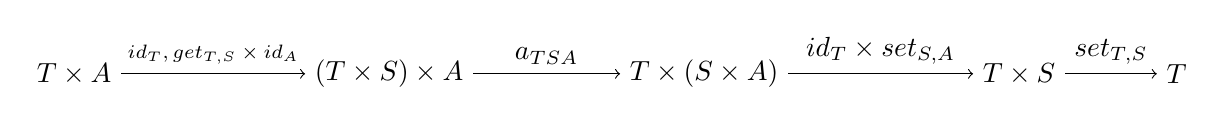
\begin{tikzpicture}[auto]
        \node (TA) at (0, 0) {$T\times A$};
        \node (TSpA) at (4, 0) {$(T\times S)\times A$};
        \node (TpSA) at (8, 0) {$T\times (S\times A)$};
        \node (TS) at (12, 0) {$T\times S$};
        \node (T) at (14, 0) {$T$};

				\draw[->] (TA) to node{\scriptsize$\tuple{id_T,get_{T,S}}\times id_A$}(TSpA);
        \draw[->] (TSpA) to node{$a_{TSA}$}(TpSA);
        \draw[->] (TpSA) to node{$id_T\times set_{S,A}$}(TS);
        \draw[->] (TS) to node{$set_{T,S}$}(T);

      \end{tikzpicture}
    \end{center}
  \end{define}
  $set_{T,A}$の定義が複雑かもしれないが、単に$T$から$S$を取り出し、$S$に$A$を与えてその$S$をまた$T$に戻しているだけである。

  またLensの合成において恒等射のような働きをするLensも定義できる。
  \begin{define}[恒等Lens]\label{def-identity-lens}
    \begin{align*}
      get_{S,S} &= id_S\\
      set_{S,S} &= \pi_{L,S\times S}
    \end{align*}
  \end{define}
  PrismにおいてもLensと同様に合成が定義できる。
  \subsection{Opticsへの一般化}
  Opticsを構成するための圏論の概念としてコエンドを定義する。
  \begin{define}[コエンド]\label{def-coend}
    ある圏$\cat{C,D}$と、関手$\functor{F}{C^{op}\times C}{D}$に対するコエンド$(\coend{C}{C} F(C,C),\kappa)$を以下のように構成する。
    \begin{quote}
      \begin{mydescription}
        \item[余楔] 余楔と呼ばれる組$(Y,\mu)$を、圏$\cat{D}$のある対象$Y$と、
        圏$\cat{C}$の任意の対象$X$に対して$\mor{\mu_C}{Y}{F(X,X)}$なる射が存在し、圏$\cat{C}$の任意の射$\mor{f}{B}{A}$に対して$\mu_A\circ F(A,f)=\mu_B\circ F(f,B)$が成り立つような$\mu$によって構成する。
        \begin{center}
          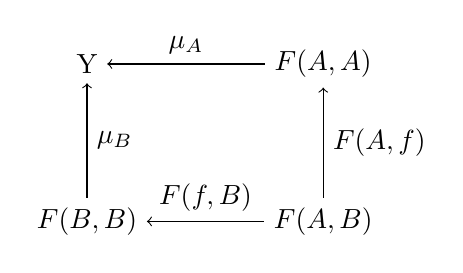
\begin{tikzpicture}[auto]
            \node (FG) at (0, 0) {Y};
            \node (FAGA) at (3, 0) {$F(A,A)$};
            \node (FBGB) at (0, -2) {$F(B,B)$};
            \node (FAGB) at (3, -2) {$F(A,B)$};
    
            \draw[<-] (FG) to node{$\mu_A$}(FAGA);  
            \draw[<-] (FG) to node{$\mu_B$}(FBGB);
            \draw[<-] (FAGA) to node{$F(A,f)$}(FAGB);
            \draw[<-] (FBGB) to node{$F(f,B)$}(FAGB);
          \end{tikzpicture}
        \end{center}
        \item[普遍性] ある余楔$(\coend{C}{C}F(C,C),\kappa)$が$F$に対してコエンドであるとは、余楔$(Y,\mu)$が存在して、任意の対象$X$において$\mu=h\circ \kappa_X$が成り立つような$\mor{h}{\coend{C}{C} F(C,C)}{Y}$が一意に存在する時である。
        また、$\kappa$を余積の場合と紛らわしくない場合は入射と呼ぶことにする。
        \begin{center}
          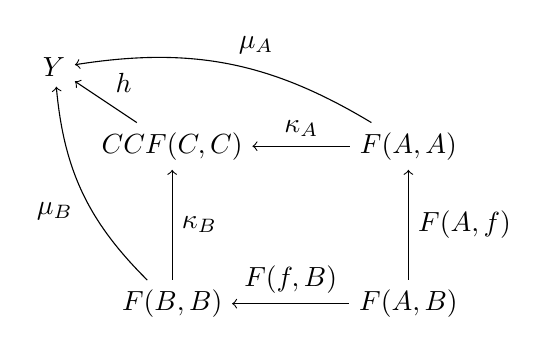
\begin{tikzpicture}[auto]
            \node (FG) at (0, 0) {$\coend{C}{C} F(C,C)$};
            \node (X) at (-1.5, 1) {$Y$};
            \node (FAGA) at (3, 0) {$F(A,A)$};
            \node (FBGB) at (0, -2) {$F(B,B)$};
            \node (FAGB) at (3, -2) {$F(A,B)$};
    
            \draw[<-] (FG) to node{$\kappa_A$}(FAGA);
            \draw[<-] (X) to node{$h$}(FG);
    
            \draw[<-] (FG) to node{$\kappa_B$}(FBGB);
            \draw[<-,bend left = 20] (X) to node{$\mu_A$}(FAGA);
            \draw[<-,bend right = 20] (X) to node[swap]{$\mu_B$}(FBGB);
            \draw[<-] (FAGA) to node{$F(A,f)$}(FAGB);
            \draw[<-] (FBGB) to node{$F(f,B)$}(FAGB);
          \end{tikzpicture}
        \end{center}
      \end{mydescription}
    \end{quote}
  \end{define}
  コエンドの普遍性は$\coend{C}{C} F(C,C)$が圏$C$の任意の対象に対する$F(C,C)$の余積であることを示していて、$F(A,B)$の元に対し$f$を$A$と$B$のどちらに適用しても入射によって示されるということである。
  
  余積という部分をもう少し詳しく見ると、$F(A,A)$から$Y$への射の族$\mu$は同様の射の族$\kappa$によって単なる射$h$へと分解される。同様に$\kappa$が他の単なる射によって分解されるかといえば、コエンドの普遍性からそのような射の族は$\kappa$以外には存在しないと言える。そういった意味で$(\coend{C}{C} F(C,C),\kappa)$は余楔の中で、射の族としての最小限の性質のみを持っていると考えられる。

  コエンドもHaskellで定義できる
  \begin{lstlisting}
    {-# LANGUAGE ExistentialQuantification #-}
    data Coend p = forall a. Coend (p a a)
    -- >>> :t Coend
    -- Coend :: p a a -> Coend p
  \end{lstlisting}
  \pr{Coend}の値コンストラクタを見ると、\pr{p a a}から\pr{Coend p}へ写る過程で型引数\pr{a}の情報を忘れてしまっている。そのため一度\pr{Coend}に写してしまうと、元の型に復元することはできなくなり、一般的には一切の操作が行えなくなってしまう。そういった意味でこれは任意の型\pr{a}で添字付けられた\pr{p a a}の直和であるように思える。

  コエンドに限らずこういった定義の手法を存在量化と呼ぶが、実用の面では最低限操作が行えることを保証するために\pr{a}の型に制約を加えることが多い。

  次にコエンドとエンドの関係性についての重要な命題を示す。
  \begin{prop}\label{prop-preservation-coend-by-hom-functor}
    \[\arset{Set}{\coend{C}{C} T(C,C)}{X}\cong\cend{C}{C}\arset{Set}{T(C,C)}{X}\]であり、$X,T$に対して自然。
  \end{prop}
  \begin{proof}
    反変Hom関手は余連続であるから余極限を保つ。またエンドは極限によって定義できるように、コエンドも余極限によって定義できる。これによってコエンドは反変Hom関手によって保たれるが、反変性よりコエンドの双対であるエンドとして保たれる。
  \end{proof}
  \begin{define}[Optics]\label{def-optics}
    対称モノイダル圏$\cat{C}$における組$(S,S')$、$(A,A')$の間のOpticの集合を
    \[Optic_\cat{C}(S,S',A,A')=\coend{C}{M}\arset{C}{S}{M\otimes A}\times \arset{C}{M\otimes A'}{S'}\]と定義する。
    また、$\kappa_M(l,r)$となる$Optic_\cat{C}(S,S',A,A')$の元を、紛らわしくない場合に$\mor{\tuple{l,r}}{(S,S')}{(A,A')}$と表記する。
    \begin{center}
      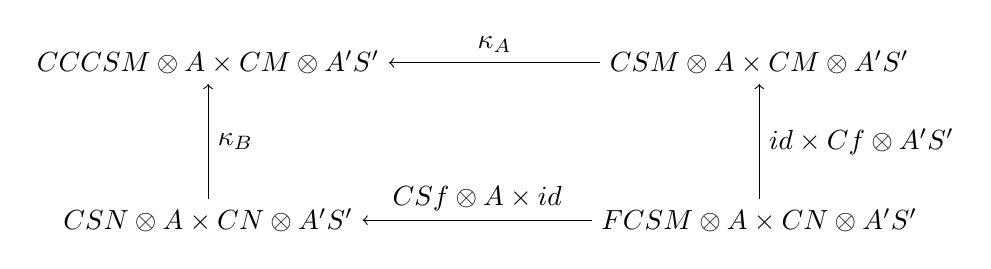
\begin{tikzpicture}[auto]
        \node (FG) at (0, 0) {$\coend{C}{C} \arset{C}{S}{M\otimes A}\times\arset{C}{M\otimes A'}{S'}$};
        \node (FAGA) at (7, 0) {$\arset{C}{S}{M\otimes A}\times\arset{C}{M\otimes A'}{S'}$};
        \node (FBGB) at (0, -2) {$\arset{C}{S}{N\otimes A}\times\arset{C}{N\otimes A'}{S'}$};
        \node (FAGB) at (7, -2) {$F\arset{C}{S}{M\otimes A}\times\arset{C}{N\otimes A'}{S'}$};

        \draw[<-] (FG) to node{$\kappa_A$}(FAGA);
        \draw[<-] (FG) to node{$\kappa_B$}(FBGB);
        \draw[<-] (FAGA) to node{$id\times\arset{C}{f\otimes A'}{S'}$}(FAGB);
        \draw[<-] (FBGB) to node{$\arset{C}{S}{f\otimes A}\times id$}(FAGB);
      \end{tikzpicture}
    \end{center}
  \end{define}
  この定義におけるコエンドの普遍性は、$\arset{C}{S}{M\otimes A}\times \arset{C}{N\otimes A'}{S'}$の元$\tuple{l,r}$に対し、
  \[\kappa_N((f\otimes A)\circ l, r)=\kappa_M(l, r(f\otimes A'))\]が成り立つような$\kappa$を入射とする$\arset{C}{S}{M\otimes A}\times \arset{C}{M\otimes A'}{S'}$の余積である。

  \begin{prop}
    任意のOptics$\kappa_M\tuple{l,r}$と、$f^{-1}\circ f = id_M$を満たす任意の射$\mor{f}{M}{N},\ \mor{f^{-1}}{N}{M}$に対して\[\kappa_M\tuple{l,r} = \kappa_N\tuple{(f\otimes A)l,r(f^{-1}\otimes A)}\]である。また$f$は必ずしも同型射である必要はない。
  \end{prop}

  次にOpticsがLens、Prismの一般化であることを示したいが、そのために余米田の補題が必要であるためここで示す。

  \begin{define}[余米田の補題]\label{def-coyoneda-lemma}
    任意の圏$\cat{C}$と対象$A$と関手$\functor{F}{C}{Set}$において
    \[FA\cong\coend{C}{C} FC\times\arset{C}{C}{A}\]
    またここでの積分記号はエンドではなくコエンドである。
  \end{define}
  \begin{proof}
    米田の原理より、\[A\cong B\iff\arset{C}{A}{-}\cong\arset{C}{B}{-}\]であるから、$\arset{Set}{FA}{X}\cong\arset{Set}{\coend{C}{C} FC\times\arset{C}{C}{A}}{X}$が$X$に対して自然に成り立つことを示せば良い。またコエンドは関手であるから、同型を保つ。
    \begin{align*}
      \arset{Set}{\coend{C}{C} FC\times\arset{C}{C}{A}}{X}&\cong\cend{C}{C}\arset{Set}{FC\times\arset{C}{C}{A}}{X}&\text{(反変Hom関手の余極限の保存)}\\
      &\cong\cend{C}{C}\arset{Set}{\arset{C}{C}{A}\times FC}{X}&\text{(積の交換)}\\
      &\cong\cend{C}{C}\arset{Set}{\arset{C}{C}{A}}{\arset{Set}{FC}{X}}&\text{(べき随伴の射集合同型)}\\
      &\cong\arset{Set}{FA}{X}&\text{(反変米田の補題)}
    \end{align*}
    よってである。計算のために使用した同型はすべて$X,F,A$に対して自然であるから、$FA\cong\coend{C}{C} FC\times\arset{C}{C}{A}$が成り立ち、$F,A$に対して自然である。
  \end{proof}
  また同様の方法で$F$に反変関手を取る場合も証明できる。
  すなわち、任意の関手$\functor{F}{C^{op}}{Set}$と対象$A$に対して
  \[FA\cong\coend{C}{C}FC\times \arset{C}{A}{C}\]が成り立つ。

  余米田の補題によれば、$FA$が$FC\times\arset{C}{C}{A}$を与える関手のコエンドとなるということであるが、具体的な入射の構成は不明である。余楔を用いた証明も思いつくが、$\cat{H}$が余積を持つことの証明のようにコエンドの元を列挙できないため、この方法では難しい。そのため厳密な証明では無いが直接同型射を構成して証明しよう。
  \begin{prop}
    $\coend{C}{C} FC\times\arset{C}{C}{A}$の任意の元$x$は入射$\kappa$によって与えられるとする。すなわち$x = \kappa_B(b,f)$となるようなある対象$B$とある元$b$、ある射$\mor{f}{B}{A}$の対$\tuple{b,f}$が一意に存在するとする。この時、$FA\cong\coend{C}{C} FC\times\arset{C}{C}{A}$が成り立つ。
  \end{prop}
  \begin{proof}
    同型射$\mor{\phi}{FA}{\coend{C}{C} FC\times\arset{C}{C}{A}}$、$\mor{\phi^{-1}}{\coend{C}{C} FC\times\arset{C}{C}{A}}{FA}$を以下のように定義する
    \begin{align*}
      \phi(a) &= \kappa_A(a,id_A)\\
      \phi^{-1}(x) &= \phi^{-1}(\kappa_B(b,f)) = Ffb
    \end{align*}
    すると、
    \begin{align*}
      \phi\circ\phi^{-1}(\kappa_B(b,f))&=\phi(Ffb)\\
      &=\kappa_A(Ffb,id_A)\\
      &=\kappa_B(b,f)&\text{(余楔の定義)}\\
      \phi^{-1}\circ\phi(a) &= \phi^{-1}(\kappa_A(a,id_A))\\
      &=a
    \end{align*}
    となるから、$\phi\circ\phi^{-1}=id,\ \phi^{-1}\circ\phi=id_{FA}$が成り立ち$FA\cong\coend{C}{C}FC\times \arset{C}{A}{C}$となる。
  \end{proof}

  同型射を具体的な構成によって定義できたため、Haskellでも定義できるようになった。
  \begin{lstlisting}
    {-# LANGUAGE ExistentialQuantification #-}
    data Coend p = forall a. Coend (p a a)

    data CoyonedaRaw f a c b = CoyonedaRaw (f c) (b -> a)
    type Coyoneda f a = Coend (CoyonedaRaw f a)

    toCoyoneda :: f a -> Coyoneda f a
    toCoyoneda x = Coend (CoyonedaRaw x id)

    fromCoyoneda ::Functor f => Coyoneda f a -> f a
    fromCoyoneda (Coend(CoyonedaRaw x y)) = fmap y x

    data CoyonedaRaw' f a c b = CoyonedaRaw' (f c) (a -> b)
    type Coyoneda' f a = Coend (CoyonedaRaw' f a)

    toCoyoneda' :: f a -> Coyoneda' f a
    toCoyoneda' x = Coend (CoyonedaRaw' x id)

    fromCoyoneda' :: Contravariant f => Coyoneda' f a -> f a
    fromCoyoneda' (Coend(CoyonedaRaw' x y)) = contramap y x
  \end{lstlisting}

  \begin{prop}\label{prop-lens-is-optics}
    $Optic_{\cat{H},\times}(S,S',A,A')$をOpticの定義のモノイダル積$\otimes$を直積型である積$\times$に置き換えたものとする。すると、
    \[Optic_{\cat{H},\times}(S,S,A,A) = Lens(S,A)\]である。
  \end{prop}
  \begin{proof}
    \begin{align*}
      \coend{C}{M}\arset{C}{S}{M\times A}\times \arset{C}{M\times A}{S}&\cong\coend{C}{M}\arset{C}{S}{M}\times \arset{C}{S}{A}\times \arset{C}{M\otimes A}{S}&\text{(共変Hom関手の積の保存)}\\
      &\cong\arset{C}{S}{A}\times \arset{C}{S\times A}{S}&\text{(余米田の補題)}\\
    \end{align*}
  \end{proof}
  同様にPrismもOpticで表せる。
  \begin{prop}\label{prop-prism-is-optics}
    \[Optic_{\cat{C},+}(S,S,A,A) = Prism(S,A)\]である。
  \end{prop}
  \begin{proof}
    \begin{align*}
      \coend{C}{M}\arset{C}{S}{M+A}\times \arset{C}{M+A}{S}&\cong\coend{C}{M}\arset{C}{S}{M+A}\times \arset{C}{M}{S}\times \arset{C}{A}{S}&\text{(反変Hom関手の余積の保存)}\\
      &\cong\arset{C}{S}{S+A}\times \arset{C}{A}{S}&\text{(余米田の補題)}\\
    \end{align*}
  \end{proof}
  この計算も具体的な操作によって行なっているため、Haskellで記述することができる。また紙面の関係上Lensのみを示す。
  \begin{lstlisting}
  coendFmap :: forall p q. (forall a. p a a -> q a a) 
  -> Coend p -> Coend q
  coendFmap f (Coend p) = Coend (f p)
  
  data Lens s a = Lens{get :: s -> a , set :: (s, a) -> s}

  opticToLens :: Optic s s a a (,) -> Lens s a
  opticToLens x = toLens $ fromCoyoneda' (coendFmap f x) where

    f :: OpticRaw s s a a (,) m n 
    -> CoyonedaRaw' (PseudoLens s a) s m n
    f (OpticRaw l r) = CoyonedaRaw' (PseudoLens (snd (outProduct l)) r)
    (fst (outProduct l)) 

    toLens :: PseudoLens s a s -> Lens s a
    toLens (PseudoLens x y) = Lens x y

  lensToOptic :: Lens s a -> Optic s s a a (,)
  lensToOptic (Lens get set) =coendFmap f 
  (toCoyoneda'(PseudoLens get set)) where

    f :: CoyonedaRaw' (PseudoLens s a) s m n -> OpticRaw s s a a (,) m n
    f (CoyonedaRaw' (PseudoLens g s) y) = OpticRaw (inProduct (y, g)) s

  data PseudoLens s a m = PseudoLens{g :: s -> a , s :: (m, a) -> s}

  instance Contravariant (PseudoLens s a) where
    contramap :: (c -> b) -> PseudoLens s a b -> PseudoLens s a c
    contramap f (PseudoLens x y) = PseudoLens x (y.first f)
  \end{lstlisting}
  ここでの\pr{coendFmap}は、双関手間の自然変換\[\natf{\alpha}{P}{Q}{H\times H}{H}\]をコエンド間の射\[\mor{\displaystyle\int\alpha}{\coend{H}{C}P(C,C)}{\coend{H}{C}Q(C,C)}\]へと写す射関数である。コエンドを取る操作が関手であることは、コエンドを構成する余極限を取る操作が関手であることからわかる。


  またこの同型によって、Lensを構成する関数$\mor{set}{S\times A}{S}$、$\mor{get}{S}{A}$からOptics$\coend{C}{M}\arset{C}{S}{M\otimes A}\times \arset{C}{M\otimes A}{S}$の値に変換するかを見ることができる。実際に逆にたどると、
  \begin{align*}
    &\tuple{get,set}&:&\arset{C}{S}{A}\times \arset{C}{S\times A}{S}\\
    \intertext{$F(M)=\arset{C}{S}{A}\times \arset{C}{M\times A}{S}$とすると、}
    =&\tuple{get,set}&:&F(S)\\
    \intertext{余米田の補題の$\phi(a)=\kappa_A(a,id_A)$より、}
    \rightarrow&\kappa_S(\tuple{get,set},id_S)&:&\coend{C}{M}F(M)\times \arset{C}{S}{M}\\
    \intertext{表記を変えて}
    =&\kappa_S(get,set,id_S)&:&\coend{C}{M}\arset{C}{S}{A}\times \arset{C}{S\times A}{S}\times \arset{C}{S}{M}\\
    \rightarrow&\kappa_S(id_S,get,set)&:&\coend{C}{M}\arset{C}{S}{M}\times\arset{C}{S}{A}\times \arset{C}{S\times A}{S}\\
    \intertext{$\mor{id_S}{S}{S}$、$\mor{get}{S}{A}$であるから射の対$\mor{\tuple{id_S,get}}{S}{S\times A}$を取って、}
    \rightarrow&\kappa_S(\tuple{id_S,get},set)&:&\coend{C}{M}\arset{C}{S}{M\times A}\times \arset{C}{M\times A}{S}
  \end{align*}
  というように$Optic(S,S,A,A)_{\cat{C},\times}$の値が得られる。ここでの$\kappa_S(\tuple{id_S,get},set)$は\[\tuple{\tuple{id_S,get},set}:\arset{C}{S}{S\times A}\times \arset{C}{S\times A}{S}\]をコエンドへ入射したものであり、Lensの場合は$M=S$となることが分かった。これにより、Opticは与えられた$S$を$\mor{l}{S}{M\otimes A}$によって$M$と$A$に分解し、$\mor{r}{M\otimes A}{S}$によって新たに与えられた$A$と、$l$によって得られた$M$からまた$S$を再構成する。といった流れになっていることが分かる。またこの解釈は\[Optic(S,S',A,A')_{\cat{C}}=\coend{C}{M}\arset{C}{S}{M\otimes A}\times \arset{C}{M\otimes A'}{S'}\]でも問題なく機能する。
  \subsection{Opticsの圏論的性質}
  Lens、Prismの合成と同様にOpticの合成\[\mor{\circ}{Optic_{\cat{C}}(S,S',A,A')\times Optic_{\cat{C}}(T,T',S,S')}{Optic_{\cat{C}}(T,T',A,A')}\]を考える。
  \begin{prop}[フビニの定理]\label{prop-fubini-theorem}
    \[\cend{C}{C}\ \ \ \ \cend{D}{D}T(C,C,D,D)\cong\cend{C\times D}{C,D}T(C,C,D,D)\]
    \[\coend{C}{C}\ \ \ \ \coend{D}{D}T(C,C,D,D)\cong\coend{C\times D}{C,D}T(C,C,D,D)\]
  \end{prop}
  \begin{proof}
    省略。エンドが右随伴関手であり、その一意性により示せる。
  \end{proof}
  \begin{prop}[積のコエンドの保存]\label{prop-preservation-of-coend-by-product}
    関手$\functor{T,S}{C^{op}\times C}{Set}$において
    \[\coend{C}{C}T(C,C)\times \coend{C}{D}S(D,D)\cong\coend{C\times C}{C,D}T(C,C)\times S(D,D)\]であり$T,S$に対して自然。
  \end{prop}
  \begin{proof}
    前提として、$\cat{Set}$においてもべき随伴$(-\times B)\dashv(-)^B$が成り立つから、$(-\times B)$は左随伴関手であり余連続である。
    \begin{align*}
      \coend{C}{C}T(C,C)\times \coend{C}{D}S(D,D)&\cong\coend{C}{C}(T(C,C)\times \coend{C}{D}S(D,D))&\text{(積関手の余連続性)}\\
      &\cong\coend{C}{C}(\coend{C}{D}S(D,D)\times T(C,C))&\text{(積関手の余連続性)}\\
      &\cong\coend{C}{C}(\coend{C}{D}T(C,C)\times S(D,D))&\text{(積の交換則)}\\
      &\cong\coend{C\times C}{C,D}T(C,C)\times S(D,D)&\text{(フビニの定理)}
    \end{align*}
  \end{proof}
  \begin{define}[Opticの合成]\label{def-comp-of-optic}
    Opticの合成{\scriptsize\[\mor{\circ}{\coend{C\times C}{M,N}\arset{C}{S}{M\otimes A}\times \arset{C}{M\otimes A'}{S'}\times \arset{C}{T}{N\otimes S}\times\arset{C}{N\otimes S'}{T'}}{\coend{C}{M\otimes N}\arset{C}{T}{(M\otimes N)\otimes A}\times \arset{C}{(M\otimes N)\otimes A'}{T'}}\]}を定義するが、コエンドの普遍性より、
    \[\mor{\circ_{MN}}{\arset{C}{S}{M\otimes A}\times \arset{C}{M\otimes A'}{S'}\times \arset{C}{T}{N\otimes S}\times\arset{C}{N\otimes S'}{T'}}{\arset{C}{T}{(M\otimes N)\otimes A}\times \arset{C}{(M\otimes N)\otimes A'}{T'}}\]
    を各$M,N$に対して$\circ_{MN}$を定義できれば$\circ$は一意に定まる。

    \[\tuple{l,r}\circ_{MN}\tuple{l',r'}=\tuple{a_{NMA}^{-1}\circ(N\otimes l)\circ l',r'\circ(N\otimes r)\circ a_{NMA'}^{-1}}\]によって$\circ$を定義する。
    \begin{center}
      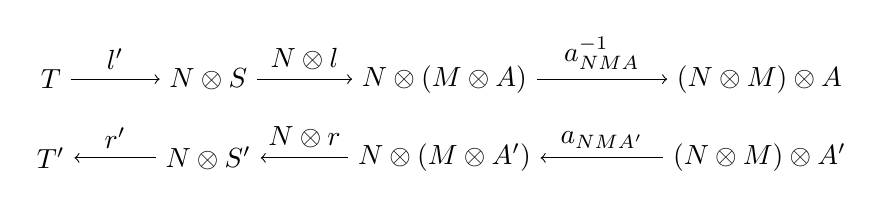
\begin{tikzpicture}[auto]
        \node (T) at (0, 0) {$T$};
        \node (NS) at (2, 0) {$N\otimes S$};
        \node (NMA) at (5, 0) {$N\otimes (M\otimes A)$};
        \node (NMA') at (9, 0) {$(N\otimes M)\otimes A$};

        \draw[->] (T) to node{$l'$}(NS);
        \draw[->] (NS) to node{$N\otimes l$}(NMA);
        \draw[->] (NMA) to node{$a_{NMA}^{-1}$}(NMA');

        \node (T) at (0, -1) {$T'$};
        \node (NS) at (2, -1) {$N\otimes S'$};
        \node (NMA) at (5, -1) {$N\otimes (M\otimes A')$};
        \node (NMA') at (9, -1) {$(N\otimes M)\otimes A'$};

        \draw[<-] (T) to node{$r'$}(NS);
        \draw[<-] (NS) to node{$N\otimes r$}(NMA);
        \draw[<-] (NMA) to node{$a_{NMA'}$}(NMA');

      \end{tikzpicture}
    \end{center}
    このようにOptic同士の合成はつなげると言うよりかは、埋め込むという印象の方が強い。
  \end{define}
  \begin{define}[恒等Optic]\label{def-identity-optic}
    任意の対象$S,S'$に対する恒等Opticを、モノイダル圏の左単位子$\mor{\lambda_S^{-1}}{S}{I\otimes S}$、$\mor{\lambda_{S'}}{I\otimes S}{S}$によって、
    \[id_{S,S'}=\kappa_I(\lambda_S^{-1},\lambda_{S'}):\coend{C}{M}\arset{C}{S}{M\otimes S}\times \arset{C}{M\otimes S'}{S'}\]と定義する。
  \end{define}
  \begin{prop}[Opticの結合則]\label{prop-associativity-of-optic}
    任意のOptic$\mor{\tuple{l,r}}{(S,S')}{(A,A')},\ \mor{\tuple{l',r'}}{(T,T')}{(S,S')},\ \mor{\tuple{l'',r''}}{(R,R')}{(T,T')}$に対して、
    \[(\tuple{l,r}\circ\tuple{l',r'})\circ\tuple{l'',r''}=\tuple{l,r}\circ(\tuple{l',r'}\circ\tuple{l'',r''})\]が成り立つ。
  \end{prop}
  \begin{proof}
    Opticの合成と同様に、フビニの定理より三つのコエンドを一つのコエンドとして計算できる。またモノイダル積関手の射の合成の保存より、適当に展開すれば簡単に示せる。
  \end{proof}
  \begin{prop}[Opticの単位元則]\label{prop-optic-has-identity}
    任意のOptic$\mor{\tuple{l,r}}{(S,S')}{(A,A')}$に対して、
    \[\tuple{\lambda_A^{-1},\lambda_{A'}}\circ\tuple{l,r}=\tuple{l,r}\]
    \[\tuple{l,r}\circ\tuple{\lambda_S^{-1},\lambda_{S'}}=\tuple{l,r}\]
    が成り立つ。
  \end{prop}
  \begin{proof}
    左単位子の振る舞いを観察するために前者は実際に示そう。
    \begin{align*}
      \tuple{\lambda_A^{-1},\lambda_{A'}}\circ\tuple{l,r}
      &=\tuple{a^{-1}_{MIA}\circ(M\otimes\lambda_A^{-1})\circ l, r\circ(M\otimes\lambda_{A'})\circ a_{MIA'}}&\text{(Opticの合成の定義)}\\
      &=\tuple{(\rho_M^{-1}\otimes A)\circ l,r\circ(\rho_M\otimes A')}&\text{(モノイダル圏の三角恒等式)}\\
      &=\tuple{l,r\circ (\rho_M\otimes A')\circ(\rho_M^{-1}\otimes A')}&\text{(余楔の定義)}\\
      &=\tuple{l,r}
    \end{align*}
    またモノイダル圏の三角恒等式を使用する場面においては$l$の方の図式を示しておく。
    \begin{center}
      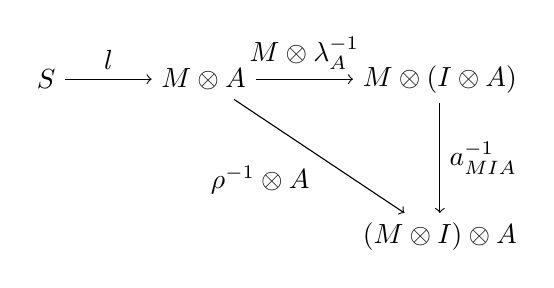
\begin{tikzpicture}[auto]
        \node (S) at (0, 0) {$S$};
        \node (MA) at (2, 0) {$M\otimes A$};
        \node (MIA) at (5, 0) {$M\otimes (I\otimes A)$};
        \node (MIA') at (5, -2) {$(M\otimes I)\otimes A$};
        \draw[->] (S) to node{$l$}(MA);
        \draw[->] (MA) to node{$M\otimes\lambda_A^{-1}$}(MIA);
        \draw[->] (MIA) to node{$a^{-1}_{MIA}$}(MIA');
        \draw[->] (MA) to node[swap]{$\rho^{-1}\otimes A$}(MIA');

      \end{tikzpicture}
    \end{center}
  \end{proof}
  これによって圏の公理をひと通り示せたから、実際にOpticsの圏が定義できる。
  \begin{define}[Opticsの圏]\label{def-cat-of-optics}
    対称モノイダル圏$\cat{C}$上の圏$\cat{Optic_C}$を以下のように定義する。
    \begin{quote}
			\begin{mydescription}
				\item[対象] 対象の集合を$\obj{Optic_C}=\obj{C}\times \obj{C}$とする。これは単に圏$\cat{C}$の対象の組である。
				\item[射] 任意の対象$(S,S'), (A,A')$に対する射集合を\[\arset{Optic_C}{(S,S')}{(A,A')}=\coend{C}{M}\arset{C}{S}{M\otimes A}\times\arset{C}{M\otimes A'}{S'}\]とする。射集合の元である射$\mor{\tuple{l,r}}{(S,S')}{(A,A')}$はそのままOpticである。
				\item[射の合成] 定義\ref{def-comp-of-optic}を射の合成とする。
				すなわち射{\scriptsize\[\mor{\circ}{\coend{C}{M}\arset{C}{S}{M\otimes A}\times \arset{C}{M\otimes A'}{S'}\times\coend{C}{N} \arset{C}{T}{N\otimes S}\times\arset{C}{N\otimes S'}{T'}}{\coend{C}{M\otimes N}\arset{C}{T}{(M\otimes N)\otimes A}\times \arset{C}{(M\otimes N)\otimes A'}{T'}}\]}を射の合成を行う写像とみなすということである。またこの写像は、ある対象$M,N$に対して
        \[\tuple{l,r}\circ_{MN}\tuple{l',r'}=\tuple{a_{NMA}^{-1}\circ(N\otimes l)\circ l',r'\circ(N\otimes r)\circ a_{NMA'}^{-1}}\]
        となるような操作だった。
				\item[恒等射の存在] 定義\ref{def-identity-optic}を恒等射とする。これも任意の対象$(S,S')$に対して\[\kappa_I(\lambda_S^{-1},\lambda_{S'}):\coend{C}{M}\arset{C}{S}{M\otimes S}\times \arset{C}{M\otimes S'}{S'}\]を恒等射とみなすということである。
				\item[結合律] 命題\ref{prop-associativity-of-optic}より、任意のOptic$\mor{\tuple{l,r}}{(S,S')}{(A,A')},\ \mor{\tuple{l',r'}}{(T,T')}{(S,S')},\ \mor{\tuple{l'',r''}}{(R,R')}{(T,T')}$に対して、
        \[(\tuple{l,r}\circ\tuple{l',r'})\circ\tuple{l'',r''}=\tuple{l,r}\circ(\tuple{l',r'}\circ\tuple{l'',r''})\]が成り立つ。
				\item[単位元律] 命題\ref{prop-optic-has-identity}より、任意のOptic$\mor{\tuple{l,r}}{(S,S')}{(A,A')}$に対して、
        \[\tuple{\lambda_A^{-1},\lambda_{A'}}\circ\tuple{l,r}=\tuple{l,r}\]
        \[\tuple{l,r}\circ\tuple{\lambda_S^{-1},\lambda_{S'}}=\tuple{l,r}\]
        が成り立つ。
			\end{mydescription}
		\end{quote}
  \end{define}
  Opticが圏になることを示したから、それらの操作がLensのものと一致することを調べる。
  \begin{prop}
    Lensの合成と、Opticを経由したLensの合成は一致する。
  \end{prop}
  \begin{proof}
    任意のLensから変換されたOptic\[\mor{\tuple{\tuple{id_S,get_{SA}},set_{SA}}}{(S,S)}{(A,A)}\]
    \[\mor{\tuple{\tuple{id_T,get_{TS}},set_{TS}}}{(T,T)}{(S,S)}\]の合成を計算し、これをLensに変換する。

    合成されたOpticにおける左側の射$l$は、
    \begin{center}
      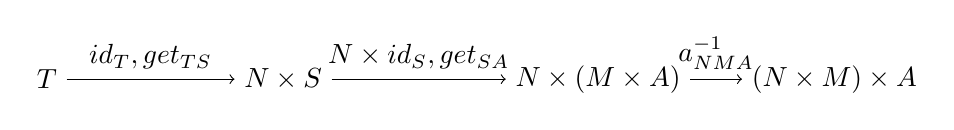
\begin{tikzpicture}[auto]

        \node (T) at (0, -1) {$T$};
        \node (NS) at (3, -1) {$N\times S$};
        \node (NMA) at (7, -1) {$N\times (M\times A)$};
        \node (NMA') at (10, -1) {$(N\times M)\times A$};

        \draw[->] (T) to node{$\tuple{id_T,get_{TS}}$}(NS);
        \draw[->] (NS) to node{$N\times \tuple{id_S,get_{SA}}$}(NMA);
        \draw[->] (NMA) to node{$a_{NMA}^{-1}$}(NMA');
      \end{tikzpicture}
    \end{center}
    \[l = a\circ(id_T\times\tuple{id_S,get_{SA}})\circ\tuple{id_T,get_{TS}}\]となるが、これは少し簡約できる。
    \begin{align*}
      &a\circ(id_T\times\tuple{id_S,get_{SA}})\circ\tuple{id_T,get_{TS}}\\
      &=a\circ\tuple{id_T,\tuple{id_S,get_{SA}\circ get_{TS}}}&\text{(射の積の定義と対の分配則)}\\
      &=a\circ\tuple{id_T,\tuple{get_{TS},get_{SA}\circ get_{TS}}}&\text{(射の対の分配則)}\\
      &=\tuple{\tuple{id_T,get_{TS}},get_{SA}\circ get_{TS}}&\text{(結合子の定義)}\\
    \end{align*}
    合成されたOpticにおける右側の射$r$は、
    \begin{center}
      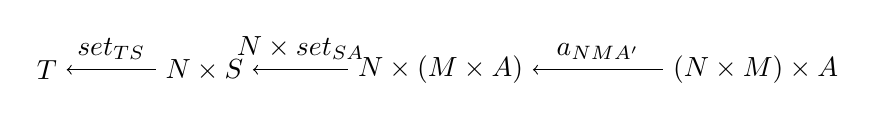
\begin{tikzpicture}[auto]
        \node (T) at (0, -1) {$T$};
        \node (NS) at (2, -1) {$N\times S$};
        \node (NMA) at (5, -1) {$N\times (M\times A)$};
        \node (NMA') at (9, -1) {$(N\times M)\times A$};

        \draw[<-] (T) to node{$set_{TS}$}(NS);
        \draw[<-] (NS) to node{$N\times set_{SA}$}(NMA);
        \draw[<-] (NMA) to node{$a_{NMA'}$}(NMA');
      \end{tikzpicture}
    \end{center}
    \[r = set_{TS}\circ\tuple{\pi_T,set_{SA}\circ\pi_{S\times A}}\circ a^{-1}\]となる。これは特に簡約できないが、元のLensの$set$の合成に類似しているため違和感は無い。
    \[\tuple{l,r}:\arset{C}{T}{(T\times S)\times A}\times\arset{C}{(T\times S)\times A}{T}\]

    次にこれをLensに復元する。命題\ref{prop-lens-is-optics}より、\[\mor{\pi_{A}\circ l=get_{SA}\circ get_{TS}}{T}{A}\]は明らかに定義\ref{def-comp-of-lens}の$get_{TA}$の定義と一致する。片方の\[\mor{\pi_{T\times S}\circ l=\tuple{id_T,get_{TS}}}{T}{T\times S}\]は$r$の$T\times S$側に合成すれば良いから、\[\mor{r\circ(\tuple{id_T,get_{TS}}\times A)}{T\times S}{T}\]
    \begin{center}
      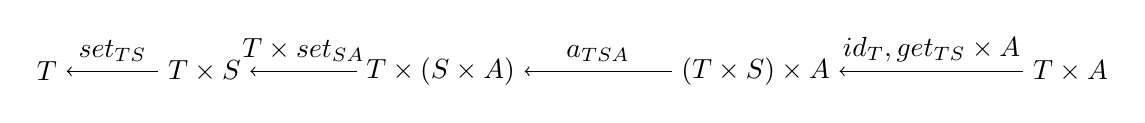
\begin{tikzpicture}[auto]
        \node (T) at (0, -1) {$T$};
        \node (NS) at (2, -1) {$T\times S$};
        \node (NMA) at (5, -1) {$T\times (S\times A)$};
        \node (NMA') at (9, -1) {$(T\times S)\times A$};
        \node (NMA'') at (13, -1) {$T\times A$};

        \draw[<-] (T) to node{$set_{TS}$}(NS);
        \draw[<-] (NS) to node{$T\times set_{SA}$}(NMA);
        \draw[<-] (NMA) to node{$a_{TSA}$}(NMA');
        \draw[<-] (NMA') to node{$\tuple{id_T,get_{TS}}\times A$}(NMA'');
      \end{tikzpicture}
    \end{center}
    となる。これが$set_{TA}$と一致するかはわかりにくいが、定義\ref{def-comp-of-lens}における$set_{TA}$の定義の図式を左右反転させたものと一致することが分かる。
  \end{proof}
  \subsection{Lawful Optics}
  LensやPrismの合成をOpticsによって一般化することができたが、それらの満たすべき制約についてもOpticsを用いて議論できる。
  例えばLensにおいて、三つのレンズ則\[\mor{\pi_A = get\circ set}{S\times A}{A}\]
  \[\mor{id_S = set\circ\tuple{id_S,get}}{S}{S\times A}\]\[\mor{set\circ(set\times A) = set\circ (\pi_S\times A)}{(S\times A)\times A}{S}\]
  を与えたが、二つ目の等式はOpticと見なした時の左右の射の合成が恒等射になっている。一つ目は恒等射とはならないものの、$get$と$set$の合成が射影射として、$A$側については恒等となっている。そのため左右の射が互いに逆射になることが条件のように思える。そのため実際に逆射となると仮定しよう。すなわち次が成り立つ。
  \[id_{S\times A} = \tuple{id_S,get}\circ set\]

  しかしこの等式が実際に成り立つとすると、
  \begin{align*}
    id_{S\times A}&=\tuple{id_S,get}\circ set\\
    &=\tuple{set,get\circ set}&\text{(射の対の分配則)}\\
    &=\tuple{set,\pi_A}&\text{(レンズ則)}\\
  \end{align*}
  $id_{S\times A}$は$\pi_S$,$\pi_A$の射の対であり、$\tuple{set,\pi_A}$と等しいから$set = \pi_S$が成り立ってしまう。このような$set$は与えられた$A$の値を完全に廃棄し、$S$の値も全く変化させないということで、完全に非直感的な操作となってしまった。これにより厳密に逆射になることを制約に加えることはできないため、少し緩めたものを考える必要がある。

  また、任意のOpticに対して逆射となるような操作を定義するには、Opticの合成と同じようにコエンドの普遍性を用いて行う必要がある。
  \begin{define}[outside関数]
    関数$\mor{outside}{\coend{C}{M}\arset{C}{S}{M\otimes A}\times\arset{C}{M\otimes A}{S}}{\arset{C}{S}{S}}$をコエンドの普遍性によって定義する。任意の対象$M$に対する射
    \[\mor{outside_M}{\arset{C}{S}{M\otimes A}\times\arset{C}{M\otimes A}{S}}{\arset{C}{S}{S}}\]を任意の射$\mor{l}{S}{M\times A},\ \mor{r}{M\otimes A}{S}$に対して\[outside(l,r)=r\circ l\]と定義する。

    次に$(\arset{C}{S}{S},outside)$が余楔であることを確認する。
    \begin{center}
      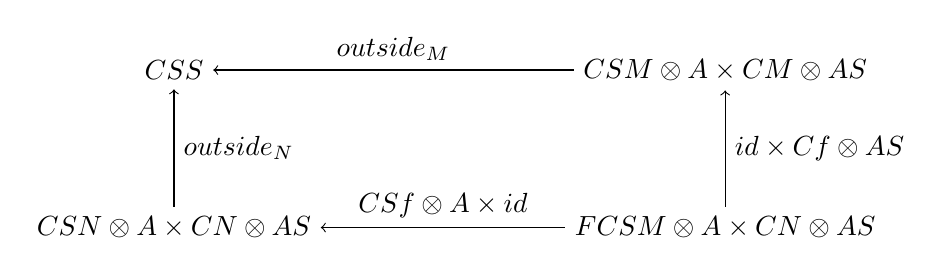
\begin{tikzpicture}[auto]
        \node (FG) at (0, 0) {$\arset{C}{S}{S}$};
        \node (FAGA) at (7, 0) {$\arset{C}{S}{M\otimes A}\times\arset{C}{M\otimes A}{S}$};
        \node (FBGB) at (0, -2) {$\arset{C}{S}{N\otimes A}\times\arset{C}{N\otimes A}{S}$};
        \node (FAGB) at (7, -2) {$F\arset{C}{S}{M\otimes A}\times\arset{C}{N\otimes A}{S}$};

        \draw[<-] (FG) to node{$outside_M$}(FAGA);
        \draw[<-] (FG) to node{$outside_N$}(FBGB);
        \draw[<-] (FAGA) to node{$id\times\arset{C}{f\otimes A}{S}$}(FAGB);
        \draw[<-] (FBGB) to node{$\arset{C}{S}{f\otimes A}\times id$}(FAGB);
      \end{tikzpicture}
    \end{center}
    任意の射$\mor{f}{N}{M},\ \mor{l}{S}{N\otimes A},\ \mor{r}{M\otimes A}{S}$に対して\[outside((f\otimes A)\circ l,r) = r\circ ((f\otimes A)\circ l)=(r\circ (f\otimes A))\circ l=outside(l,r\circ (f\otimes A))\]であるから確かに余楔である。よって\[\mor{outside}{\coend{C}{M}\arset{C}{S}{M\otimes A}\times\arset{C}{M\otimes A}{S}}{\arset{C}{S}{S}}\]はコエンドの普遍性によって一意に定まる。
  \end{define}
  
  \begin{define}[once、twice関数]
    コエンド\[Optic^2_\cat{C}(S,S,A,A)=\coend{C\times C}{M,N}\arset{C}{S}{M\otimes A}\times\arset{C}{M\otimes A}{N\otimes A}\times\arset{C}{N\otimes A}{S}\]
    に対して射$\mor{once,twice}{Optic_\cat{C}(S,S,A,A)}{Optic^2_\cat{C}(S,S,A,A)}$を定義する。

    任意の対象$M$に対して、
    \begin{align*}
      once_M(l,r) &= \tuple{l,id_{M\otimes A},r}\\
      twice_M(l,r) &= \tuple{l,l\circ r,r}
    \end{align*}
    とすると、コエンドの普遍性より$once,twice$関数は一意に定まる。
  \end{define}
  また$Optic^2_\cat{C}(S,S,A,A)$のコエンドの普遍性により、任意の射\[\mor{l}{S}{M\otimes A},\ \mor{c}{M'\otimes A}{N\otimes A},\ \mor{r}{N'\otimes A}{S}\]\[\mor{f}{M'}{M}\ \mor{g}{N'}{N}\]に対して、
  \begin{align*}
    \tuple{(f\otimes A)\circ l,c,r}&=\tuple{l,c\circ(f\otimes A),r}\\
    \tuple{l,c,r\circ(g\otimes A)} &= \tuple{l,(g\otimes A)\circ c,r}
  \end{align*}
  が成り立つ。
  \begin{define}[lawful性]
    あるOptic $\mor{\tuple{l,r}}{(S,S)}{(A,A)}$がlawfulであるとは、
    \[outside(l,r)=id_S,\ once(l,r)=twice(l,r)\]を満たす時である。
    すなわち\[r\circ l = id_S,\ \tuple{l,id_{M\otimes A},r}=\tuple{l,l\circ r,r}\]である。
  \end{define}
  outside関数による制約は単なる逆射の定義の一部であるが、once関数、twice関数による制約がどのように緩められているかについて考える。\\

  当然$\tuple{l,id_{M\otimes A},r}=\tuple{l,l\circ r,r}$ならば$id_{M\otimes A}=l\circ r$が成り立つとは限らない。これらが単なる射集合の順序対であれば成り立つが、右辺左辺はコエンドの元である。これにより余楔の等式によってこの等式が構成されていた場合は、左右の$l,r$に干渉してしまうからである。

  
  % \begin{define}[inside関数]
  %   関手$\functor{\arset{C}{M\otimes -}{M\otimes -}}{C^{op}\times C}{Set}$に対するコエンド$\coend{C}{M}\arset{C}{M\otimes A}{M\otimes A}$を用いて、ある$M$に対するある射$\mor{\phi}{M}{M}$を表現する。

  %   これによってinside関数\[\mor{inside}{\coend{C}{M}\arset{C}{S}{M\otimes A}\times\arset{C}{M\otimes A}{S}}{\coend{C}{M}\arset{C}{M\otimes A}{M\otimes A}}\]を同様にコエンドの普遍性によって定義しよう。

  %   任意の対象$M$に対して\[\mor{inside_M}{\arset{C}{S}{M\otimes A}\times\arset{C}{M\otimes A}{S}}{\arset{C}{M\otimes A}{M\otimes A}}\]を
  %   \[inside_M(l,r)=l\circ r\]とすると、コエンドの普遍性により$inside$関数が一意に定まる。
  % \end{define}
  % この二つの関数によって、定義\ref{def-lawful-optic}におけるlawful opticの等式は以下のように置き換えられる。
  % \[outside(l,r)=id_S\]
  % \[inside(l,r)=\phi\otimes A\]
  % またコエンドの普遍性によれば自明であるが以下の命題が成り立つ。
  % \begin{prop}
  %   任意のOptic $\mor{\tuple{l,r}}{(S,S)}{(A,A)}$と$f^{-1}\circ f = id_M$を満たす任意の射$\mor{f}{M}{N},\ \mor{f^{-1}}{N}{M}$に対して\begin{align*}
  %     inside(l,r)&=(f^{-1}\otimes A)\circ inside(l,r)\circ(f\otimes A)
  %   \end{align*}
  %   である。
  % \end{prop}
  % これによって、$inside(l,r)=\phi\otimes A$なる$\phi$の始域と終域は、$l,r$の始域、終域となる対象$M$と一致している必要性は無い。

  % \begin{define}[lawful Optic]\label{def-lawful-optic}
  %   あるOptic $\mor{\tuple{l,r}}{(S,S)}{(A,A)}$がlawfulであるとは、何らかの対象$M$と射$\mor{\phi}{M}{M}$が存在して
  %   \[r\circ l = id_S\]
  %   \[\tuple{l,id_A,r}\]が成り立つ時である。
  % \end{define}
  \begin{prop}[LensのLawful性]
    レンズ則を満たすLens $(get,set)$に対して、対応するOptic $\tuple{\tuple{id_S,get},set}$はLawful性を満たす。
  \end{prop}
  \begin{proof}
    Lawful性は逆射の関係と比べて、$l\circ r=id_{M\otimes A}$の条件が余楔の等式によって緩められている。そのため証明には$(-)\times A$の形の射に変形することが重要である。分かりやすい例で言えば三つ目のレンズ則
    \[set\circ(set\times A) = set\circ (\pi_S\times A)\]が該当する。また、Lensにおける合成$l\circ r$においても、
    \begin{align*}
      \tuple{id_S,get}\circ set &=\tuple{set,get\circ set}&\text{(射の対の分配則)}\\
      &=\tuple{set,\pi_A}&\text{(レンズ則)}\\
      &= (set\times A)\circ\tuple{id_{S\times A},\pi_A}&\text{(射の積の定義)}\\
    \end{align*}
    が成り立つ。これによって、
    \begin{align*}
      &\tuple{\tuple{id_S,get},\tuple{id_S,get}\circ set, set}\\
      &=\tuple{\tuple{id_S,get},(set\times A)\circ\tuple{id_{S\times A},\pi_A}, set}\\
      &=\tuple{\tuple{id_S,get},\tuple{id_{S\times A},\pi_A}, set\circ(set\times A)}&\text{(余楔の定義)}\\
      &=\tuple{\tuple{id_S,get},\tuple{id_{S\times A},\pi_A}, set\circ(\pi_S\times A)}&\text{(レンズ則)}\\
      &=\tuple{\tuple{id_S,get},(\pi_S\times A)\circ\tuple{id_{S\times A},\pi_A}, set}&\text{(余楔の定義)}\\
      &=\tuple{\tuple{id_S,get},\tuple{\pi_S,\pi_A}, set}&\text{(射の積の定義)}\\
      &=\tuple{\tuple{id_S,get},id_{S\times A}, set}&\text{(積の普遍性)}
    \end{align*}
    となり、Lens則を満たす場合はLawful性を満たすことが分かった。
  \end{proof}
  \begin{prop}[lawful性の合成における閉性]
    二つのLawful Optic \[\mor{\tuple{l,r}}{(S,S)}{(A,A)},\ \mor{\tuple{l',r'}}{(T,T)}{(S,S)}\]の合成\[\mor{\tuple{l',r'}\circ\tuple{l,r}}{(T,T)}{(A,A)}\]もまたLawfulである。
  \end{prop}
  \begin{proof}
    \[\tuple{l',r'}\circ\tuple{l,r}=\tuple{a^{-1}\circ(N\otimes l)\circ l',\ r'\circ(N\otimes r)\circ a}\]であったから、
    \[r'\circ(N\otimes r)\circ a\circ a^{-1}\circ(N\otimes l)\circ l'=id_T\]
    \begin{alignat*}{2}
      \tuple{&a^{-1}\circ(N\otimes l)\circ l',\ &a^{-1}\circ(N\otimes l)\circ l'\circ r'\circ(N\otimes r)\circ a,\ &r'\circ(N\otimes r)\circ a}\\
      =\tuple{&a^{-1}\circ(N\otimes l)\circ l',\ &id_{(N\otimes M)\otimes A},\ &r'\circ(N\otimes r)\circ a}
    \end{alignat*}
    の二つを示せば良い。ただし前者は自明であるため省略する。
    \[f_l = a^{-1}\circ(N\otimes l), \ g_r = (N\otimes r)\circ a\]とすると、後者の等式は\[\tuple{f_l\circ l',f_l\circ l'\circ r'\circ g_r, r'\circ g_r}=\tuple{f_l\circ l',f_l\circ id_{(N\otimes M)\otimes A}\circ g_r, r'\circ g_r}\]と表せる。
    余楔の等式を用いて\[\tuple{l',l'\circ r', r'} = \tuple{l', id_{N\otimes S}, r'}\]が証明できたから、この等式においても余楔の等式が成り立てば良い。すなわち\[\tuple{f_l\circ(\phi\otimes S) \circ l',f_l\circ l'\circ r'\circ g_r, r'\circ g_r} = \tuple{f_l\circ l',f_l \circ l'\circ r'\circ(\phi\otimes S)\circ g_r, r'\circ g_r}\]である。もし$\phi\otimes S$が$f_l$より外側に来れば、この組全体の余楔の等式により、$l',r'$に対しても余楔の等式が成り立つ。よって\[f_l\circ(\phi\otimes S) = ((\phi\otimes M)\otimes A)\circ f_l\]\[(\phi\otimes S)\circ g_r = g_r\circ((\phi\otimes M)\otimes A)\]を示せば良い。特に前者を図式で表すと以下のようになる。

    \begin{center}
      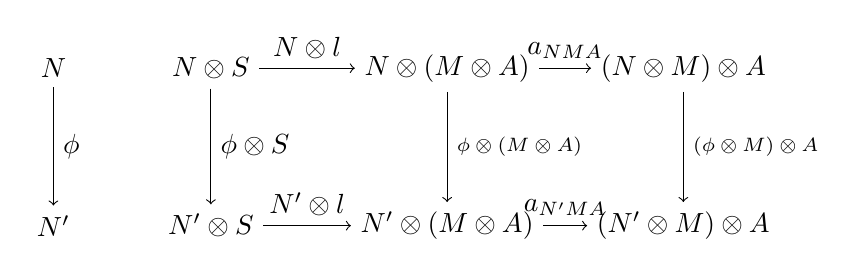
\begin{tikzpicture}[auto]
        \node (n) at (-2, 0) {$N$};
        \node (n') at (-2, -2) {$N'$};
        \draw[->] (n) to node{$\phi$}(n');

        \node (ns) at (0, 0) {$N\otimes S$};
        \node (n's) at (0, -2) {$N'\otimes S$};
        \draw[->] (ns) to node{$\phi\otimes S$}(n's);


        \node (nma) at (3, 0) {$N\otimes (M\otimes A)$};
        \node (n'ma) at (3, -2) {$N'\otimes (M\otimes A)$};
        \draw[->] (nma) to node{\scriptsize$\phi\otimes(M\otimes A)$}(n'ma);


        \node (nma2) at (6, 0) {$(N\otimes M)\otimes A$};
        \node (n'ma2) at (6, -2) {$(N'\otimes M)\otimes A$};
        \draw[->] (nma2) to node{\scriptsize$(\phi\otimes M)\otimes A$}(n'ma2);
        \draw[->] (ns) to node{$N\otimes l$}(nma);
        \draw[->] (n's) to node{$N'\otimes l$}(n'ma);
        \draw[->] (nma) to node{$a_{NMA}$}(nma2);
        \draw[->] (n'ma) to node{$a_{N'MA}$}(n'ma2);
      \end{tikzpicture}
    \end{center}
    左の正方形はモノイダル積$\otimes$の双関手性によって可換になり、右の正方形は結合子$a$の自然性によって可換になるから、全体が可換になり、\[f_l\circ(\phi\otimes S) = ((\phi\otimes M)\otimes A)\circ f_l\]が成り立つ。同様に\[(\phi\otimes S)\circ g_r = g_r\circ((\phi\otimes M)\otimes A)\]も成り立つ。これと余楔の等式によって\[\tuple{f_l\circ(\phi\otimes S) \circ l',f_l\circ l'\circ r'\circ g_r, r'\circ g_r} = \tuple{f_l\circ l',f_l \circ l'\circ r'\circ(\phi\otimes S)\circ g_r, r'\circ g_r}\]もまた成り立って、同様に\[\tuple{f_l \circ l',f_l\circ l'\circ r'\circ g_r, r'\circ g_r\circ(\phi\otimes S)} = \tuple{f_l\circ l',f_l \circ(\phi\otimes S)\circ l'\circ r'\circ g_r, r'\circ g_r}\]もまた成り立つから、\[\tuple{l',l'\circ r', r'} = \tuple{l', id_{N\otimes S}, r'}\]と同様に余楔の等式を利用して\[\tuple{f_l\circ l',f_l\circ l'\circ r'\circ g_r, r'\circ g_r}=\tuple{f_l\circ l', f_l\circ g_r, r'\circ g_r}\]というように少し簡約できた。ここからの証明も\[\tuple{l,l\circ r, r} = \tuple{l, id_{M\otimes A}, r}\]の証明と同様の操作が行えることを自然性やら関手性で示せば証明できる。
    よって    \begin{alignat*}{2}
      \tuple{&a^{-1}\circ(N\otimes l)\circ l',\ &a^{-1}\circ(N\otimes l)\circ l'\circ r'\circ(N\otimes r)\circ a,\ &r'\circ(N\otimes r)\circ a}\\
      =\tuple{&a^{-1}\circ(N\otimes l)\circ l',\ &id_{(N\otimes M)\otimes A},\ &r'\circ(N\otimes r)\circ a}
    \end{alignat*}が成り立ち、$\tuple{l',r'}\circ\tuple{l,r}$はLawfulである。
    % まず$Optic^2$同士の合成\[\mor{\circ}{Optic^2_\cat{C}(T,T,S,S)\times Optic^2\cat{C}(S,S,A,A)}{Optic^2_\cat{C}(T,T,A,A)}\]を定義しよう。
    % これは\[f_l = a^{-1}\circ(N\otimes l), \ g_r = (N\otimes r)\circ a\]として
    % \[\circ_{MN} (\tuple{l',c',r'},\tuple{l,c,r}) =\tuple{f_l\circ l',f_l\circ c'\circ g_r, r'\circ g_r}\]を任意の対象$M,N$に対して定義しコエンドの普遍性より、実際にOptic間の写像となる。
    % またこの時明らかに\[\circ (twice(l',r'),twice(l,r)) = twice(\tuple{l',r'}\circ\tuple{l,r})\]である。ここで左の引数をonce関数に置き換えると
    % \begin{align*}
    %   \circ (once(l',r'),twice(l,r)) &=  \tuple{f_l\circ l',f_l\circ g_r, r'\circ g_r}\\
    %   &=\tuple{a^{-1}\circ(N\otimes l)\circ l',\ a^{-1}\circ(N\otimes l)\circ(N\otimes r)\circ a,\ r'\circ(N\otimes r)\circ a}\\
    %   &=\tuple{a^{-1}\circ(N\otimes l)\circ l',\ a^{-1}\circ(N\otimes (l\circ r))\circ a,\ r'\circ(N\otimes r)\circ a}
    % \end{align*}
    
  \end{proof}
  \begin{prop}[恒等Opticのlawful性]  
    任意の対象$(S,S)$に対する恒等Optic$\tuple{\lambda_S^{-1},\lambda_S}$はLawfulである。
  \end{prop}
  \begin{proof}
    $\lambda_S$と$\lambda_S^{-1}$は互いに逆射であるから明らかにlawfulである。
  \end{proof}
  \section{Profunctor Optics}
  \subsection{超自然変換}
  評価射$\mor{ev_{A,B}}{A^B\times B}{A}$は$A$に対して自然であったが、$B$に対してはドメイン側に$B$が二回出ているため自然性は定義できず、代わりに超自然性を使う必要があると説明したがそれを厳密に議論する。

  \begin{define}
    関手$\functor{F}{C^{op}\times C}{Set}$に対して対象$X$、$\mor{\mu_A}{X}{T(A,A)}$が楔$(X,\mu)$である時、$\mu$を超自然変換と呼ぶ。
    また対象$X$、$\mor{\mu_A}{T(A,A)}{X}$が余楔$(X,\mu)$である時も同様に超自然変換と呼ぶ。
  \end{define}
  \begin{center}
    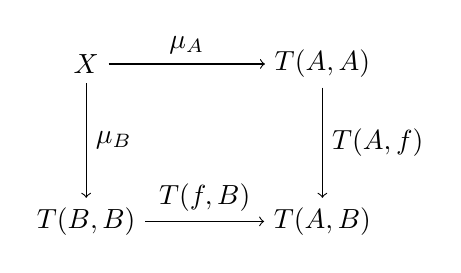
\begin{tikzpicture}[auto]
      \node (FG) at (0, 0) {$X$};
      \node (FAGA) at (3, 0) {$T(A,A)$};
      \node (FBGB) at (0, -2) {$T(B,B)$};
      \node (FAGB) at (3, -2) {$T(A,B)$};

      \draw[->] (FG) to node{$\mu_A$}(FAGA);
      \draw[->] (FG) to node{$\mu_B$}(FBGB);
      \draw[->] (FAGA) to node{$T(A,f)$}(FAGB);
      \draw[->] (FBGB) to node{$T(f,B)$}(FAGB);
    \end{tikzpicture}
  \end{center}
  自然変換がエンドで定義されることから、自然変換の成分を元と見なした時これらは超自然性を持つ。
  \begin{center}
    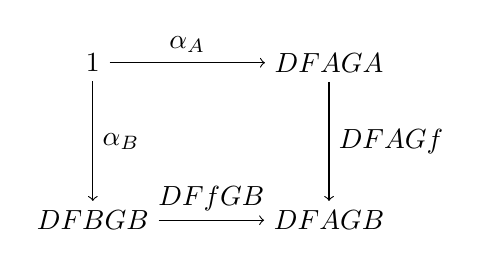
\begin{tikzpicture}[auto]
      \node (FG) at (0, 0) {$1$};
      \node (FAGA) at (3, 0) {$\arset{D}{FA}{GA}$};
      \node (FBGB) at (0, -2) {$\arset{D}{FB}{GB}$};
      \node (FAGB) at (3, -2) {$\arset{D}{FA}{GB}$};

      \draw[->] (FG) to node{$\alpha_A$}(FAGA);
      \draw[->] (FG) to node{$\alpha_B$}(FBGB);
      \draw[->] (FAGA) to node{$\arset{D}{FA}{Gf}$}(FAGB);
      \draw[->] (FBGB) to node{$\arset{D}{Ff}{GB}$}(FAGB);
    \end{tikzpicture}
  \end{center}
  \begin{prop}[評価射の超自然性]
    圏$\cat{Set}$における評価射$\mor{ev_{A,B}}{\arset{Set}{B}{A}\times B}{A}$は$A$に対して自然であったが、$B$に対しては超自然になる。
  \end{prop}
  \begin{proof}
    任意の射$\mor{g}{B'}{A}$、$\mor{f}{B}{B'}$、$B$の任意の元$b$に対して、\[ev_{A,B'}\circ\tuple{g,f(b)} = (g\circ f)(b)=ev_{A,B}\circ\tuple{g\circ f,b}\]であるから、$(A,ev_A)$は明らかに余楔となる。
    \begin{center}
      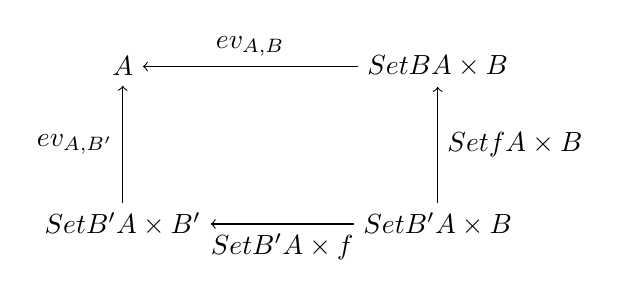
\begin{tikzpicture}[auto]
        \node (FG) at (0, 0) {$A$};
        \node (FAGA) at (4, 0) {$\arset{Set}{B}{A}\times B$};
        \node (FBGB) at (0, -2) {$\arset{Set}{B'}{A}\times B'$};
        \node (FAGB) at (4, -2) {$\arset{Set}{B'}{A}\times B$};
  
        \draw[<-] (FG) to node{$ev_{A,B}$}(FAGA);
        \draw[<-] (FG) to node[swap]{$ev_{A,B'}$}(FBGB);
        \draw[<-] (FAGA) to node{$\arset{Set}{f}{A}\times B$}(FAGB);
        \draw[<-] (FBGB) to node[swap]{$\arset{Set}{B'}{A}\times f$}(FAGB);
      \end{tikzpicture}
    \end{center}
  \end{proof}
  このコエンドの図式は余米田の補題で示したものと非常に似ているが、実際に$F=Id_{\cat{Set}}$とすると明らかに\[A\cong\coend{C}{C}\arsetr{Set}{C}{A}\times C\]が成り立つ。つまり余楔$(A,ev_A)$はコエンドでもある。
  \subsection{Profunctor}
  ProfunctorはDistributor、Relatorなどとも呼ばれている概念で、二項関係の圏論的な一般化である。

  まず集合$A,B$の間の二項関係$R$は$A\times B$の部分集合であるから、$2 = \{0,1\}$として特性関数\[\mor{R}{A\times B}{2}\]と表せる。

  また集合$2$は、ある集合$A$の二つの元を取ったときに、二つの関係は等しいか等しくないかの情報しか無く、$2$の元が二つであるのはこの情報を表すためであると考えることもできる。

  つまり二項関係では二つの集合の垣根を超えて、等しいか等しくないかの関係付けを行なっているとみなせる。これを圏に一般化しようとすると、二つの対象の間の関係は集合の圏に属する射集合で表されるから、集合$2$の代わりに圏$\cat{Set}$を使うのが望ましい。よってProfunctorは以下のように定義される。

  % 集合$A,B$の間の二項関係$R$が$A$から$B$への写像であるとは、以下の二つの条件を満たす時である。
  % \begin{quote}
  %   \begin{mydescription}
  %     \item[左全域性] $A$の任意の元$a$に対して$B$のある元$b$が存在し$aRb$である。
  %     \item[右一意性] $A$の任意の元$a$に対して、$aRb$かつ$aRb'$なる$b,b'$が存在する時$b = b'$である。 
  %   \end{mydescription}
  % \end{quote}
  % 写像$\mor{f}{A}{B}$の視点で二項関係$R$を見ると、写像と違って任意の$a$に対して、必ずしも対応する$B$の元が存在する必要はなく、かつ対応する$B$の元は必ずしも一意である必要がないということである。
  % この性質から二項関係$R$は$2 = \{0,1\}$として\[\mor{R}{A}{2^{B}}\]と表せる。またここでの$2^{B}$は特性関数の集合であるから、$B$の冪集合と同型である。

  \begin{define}[Profunctor]
    圏$\cat{A,B}$において、関手$\functor{F}{A^{op}\times B}{Set}$をProfunctorとする。
    
    また$\cat{Cat}$はカルテジアン閉圏であるから、$\functor{F}{A^{op}\times B}{Set}$と$\functor{F}{B}{\funccat{A^{op}}{Set}}$と同一視できる。
  \end{define}
  また双Hom関手$\functor{\arset{C}{-}{-}}{C^{op}\times C}{Set}$は明らかにProfunctor\ $\profunctor{\arset{C}{-}{-}}{C}{C}$である。
  \begin{define}[Profunctorの合成]
    Profunctor\ $\profunctor{F}{A}{B},\ \profunctor{G}{B}{C}$の合成
    $\profunctor{G\diamond F}{A}{C}$を
    \[(G\diamond F)(A,C) = \coend{B}{B} G(B, C)\times F(A, B)\]と定義する。
  \end{define}
  集合の圏においてコエンドは添字付けられた余積のように働いたから、$(G\diamond F)(A,C)$は大まかには$\cat{B}$の任意の対象$B$に対する$G(B,C)$と$F(A,B)$の元の組をすべて含むような集合とみなすことができる。
  \begin{prop}[Profunctorの結合律]
    \[(H\diamond G)\diamond F \cong H\diamond(G\diamond F)\]
  \end{prop}
  \begin{prop}[Profunctorの単位元律]
    \[F\diamond \arset{A}{-}{-} \cong F,\ \arset{B}{-}{-}\diamond F\cong F\]
  \end{prop}

  またHaskellにおける\pr{Profunctor}型クラスのインスタンス\pr{f}は$\functor{f}{H^{op}\times H}{H}$であるから
  \begin{lstlisting}
    class Profunctor p where
      dimap :: (a -> b) -> (c -> d) -> p b c -> p a d
      dimap f g = lmap f . rmap g
  \end{lstlisting}
  と定義できる。またProfunctor同士の合成は
  \begin{lstlisting}
    data CompRaw q p a c b d = CompRaw (q b c, p a d)
    newtype Comp q p a c = Comp (Coend (CompRaw q p a c))

    (<>) :: (Profunctor p , Profunctor q) =>
     q b c -> p a b -> Comp q p a c
    (<>) q p = Comp (Coend (CompRaw (q , p)))

    instance (Profunctor p, Profunctor q) => Profunctor(Comp q p) where
      dimap :: (Profunctor p, Profunctor q) =>
       (a -> b) -> (c -> d) -> Comp q p b c -> Comp q p a d
      dimap f g (Comp(Coend (CompRaw (q, p)))) = 
      Comp(Coend(CompRaw (rmap g q, lmap f p)))
  \end{lstlisting}
  ProfunctorによってどのようにOpticsが一般化されるかを紹介するために次の命題を予め載せる。
  \begin{prop}[Opticsの表現可能定理]
    \[\cend{Tamb}{P}\arset{Set}{P(A,A')}{P(S,S')}\cong Optics_\cat{C}(S,S',A,A')\]
  \end{prop}
  $P$が属する圏$\cat{Tamb}$は丹原加群の圏であり、$P$は特殊なProfunctorである。
  $P$についてもう少し説明すると、
  まずモノイダル積関手$\mor{M\otimes -}{C}{C}$における射関数は\[\mor{M\otimes -}{\arset{C}{A}{A'}}{\arset{C}{M\otimes A}{M\otimes A'}}\]というような射であるが、これを双Hom関手$\functor{\arset{C}{-}{-}}{C^{op}\times C}{Set}$から拡張して\[\mor{\zeta_{A,A',M}}{P(A,A')}{P(M\otimes A, M\otimes A')}\]となるような射を考える。またモノイダル積関手の射関数では、射関数の自然性から$A,A'$に対して自然であったから$\zeta$にも$A,A'$に対する自然性を課す。さらに射$\mor{f}{M}{N}$に対してモノイダル積関手の間の自然変換$\nat{f\otimes -}{M\otimes -}{N\otimes -}$を考えることができたから、その成分に該当する$\zeta$にも$M$に対する自然性を課したい。しかし$P(M\otimes A,M\otimes A')$や$P(N\otimes A, N\otimes A')$は射集合ではないから代わりに超自然性を課す。

  

  \begin{center}
    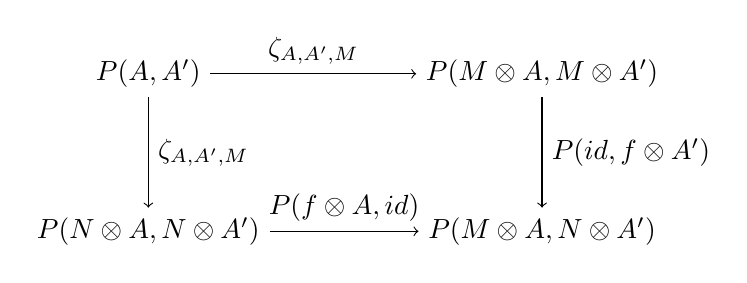
\begin{tikzpicture}[auto]
      \node (FG) at (0, 0) {$P(A,A')$};
      \node (FAGA) at (5, 0) {$P(M\otimes A,M\otimes A')$};
      \node (FBGB) at (0, -2) {$P(N\otimes A,N\otimes A')$};
      \node (FAGB) at (5, -2) {$P(M\otimes A,N\otimes A')$};

      \draw[->] (FG) to node{$\zeta_{A,A',M}$}(FAGA);
      \draw[->] (FG) to node{$\zeta_{A,A',M}$}(FBGB);
      \draw[->] (FAGA) to node{$P(id,f\otimes A')$}(FAGB);
      \draw[->] (FBGB) to node{$P(f\otimes A,id)$}(FAGB);
    \end{tikzpicture}
  \end{center}
  \begin{define}[丹原加群の圏]
    対称モノイダル圏$\cat{C}$に対する圏$\cat{Tamb}$を以下のように定義する。
    \begin{quote}
			\begin{mydescription}
				\item[対象] Profunctor\ $\profunctor{P}{C}{C}$と自然変換$\zeta$の組$(P,\zeta)$
				\item[射]対象$(P,\zeta)$、$(Q,\eta)$の間の射を、
          
				\item[射の合成]
				\item[恒等射の存在]
				\item[結合律]
				\item[単位元律]
			\end{mydescription}
		\end{quote}
  \end{define}
\end{document}
・TaPL
・私が書いた圏論入門
・すごいH本
・https://hackage.haskell.org/
・basic concept of enriched category theory
・distributer at works


https://www.cs.ox.ac.uk/jeremy.gibbons/publications/proyo.pdf
https://hackage.haskell.org/package/optics-0.4.2/docs
https://arxiv.org/pdf/2001.07488.pdf
https://arxiv.org/pdf/1809.00738.pdf
https://arxiv.org/pdf/1501.02503.pdf (coend calculus)
https://bartoszmilewski.com/2017/03/29/ends-and-coends/
https://github.com/BartoszMilewski/Publications/blob/master/TheDaoOfFP/DaoFP.pdf
dont fear profunctor optics
タイトル 圏論側からの方向性 圏論の概念
現在だとデザイン
総合報告まとめ

int型はint値の集合

todo

グローバル
・元の対を\tupleではなく()で表す

ローカル
・prismの第三法則を追加
・lens則、prism則に名前をつける
・関数名の字体を揃える
・文章中ではレンズ、プリズムのように表記する
・コエンド、余積の証明にSetを用いる。
・SetとHがゴチャゴチャになっている